\documentclass[11pt,a4paper]{ivoa}
\input tthdefs

\usepackage{todonotes}
\usepackage{listings}
\lstloadlanguages{XML}
\lstset{flexiblecolumns=true,tagstyle=\ttfamily, showstringspaces=False}

\title{VOResource: an XML Encoding Schema for Resource Metadata}

\ivoagroup{Registry}

\author[http://www.ivoa.net/twiki/bin/view/IVOA/RayPlante]{Raymond Plante}
\author[http://www.ivoa.net/twiki/bin/view/IVOA/KevinBenson]{Kevin Benson}
\author[http://www.ivoa.net/twiki/bin/view/IVOA/MarkusDemleitner]{Markus Demleitner}
\author[http://www.ivoa.net/twiki/bin/view/IVOA/MatthewGraham]{Matthew Graham}
\author[http://www.ivoa.net/twiki/bin/view/IVOA/GretchenGreene]{Gretchen Greene}
\author[http://www.ivoa.net/twiki/bin/view/IVOA/PaulHarrison]{Paul Harrison}
\author[http://www.ivoa.net/twiki/bin/view/IVOA/GerardLemson]{Gerard Lemson}
\author[http://www.ivoa.net/twiki/bin/view/IVOA/TonyLinde]{Tony Linde}
\author[http://www.ivoa.net/twiki/bin/view/IVOA/GuyRixon]{Guy Rixon}

\editor{Ray Plante, Markus Demleitner}

\previousversion[http://www.ivoa.net/Documents/REC/ReR/VOResource-20080222.html]{REC -1.03}
\previousversion[http://www.ivoa.net/Documents/WD/ReR/VOResource-20061107.html]
  {WD 2006-11-07}
\previousversion[http://www.ivoa.net/Documents/WD/ReR/VOResource-20060620.html]
  {WD 2006-06-20}
\previousversion[http://www.ivoa.net/Documents/WD/ReR/VOResource-20060530.html]
  {WD-2006-05-30}
      

\begin{document}
\begin{abstract}
This document describes an XML encoding standard for IVOA Resource
Metadata, referred to as VOResource.  This schema is primarily
intended to support interoperable registries used for discovering
resources; however, any application that needs to describe resources
may use this schema.  In this document, we define the types and
elements that make up the schema in close alignment to the metadata terms
defined in Resource Metadata for the Virtual Observatory
\citep{2007ivoa.spec.0302H}, but also taking into account other metadata
standards as well as experiences from the operation of the VO Registry.
We also describe the general model for the
schema and explain how it may be extended to add new metadata terms and
describe more specific types of resources.  
\end{abstract}


\section*{Acknowledgments}

This document has been developed with support from the
National Science Foundation's
Information Technology Research Program under Cooperative Agreement
AST0122449 with The Johns Hopkins University, from the
UK Particle Physics and Astronomy
Research Council (PPARC), and from the
European Commission's Sixth
Framework Program via the 
Optical Infrared Coordination Network (OPTICON).  Funding for the 2016
update was provided by BMBF grant GAVO-2014, grant number 05A14VHA.

The vocabulary management closely follows what Norman Gray  has
developed for Datalink.

\section*{Conformance-related definitions}

The words ``MUST'', ``SHALL'', ``SHOULD'', ``MAY'', ``RECOMMENDED'', and
``OPTIONAL'' (in upper or lower case) used in this document are to be
interpreted as described in IETF standard RFC2119 \citep{std:RFC2119}.

The \emph{Virtual Observatory (VO)} is a
general term for a collection of federated resources that can be used
to conduct astronomical research, education, and outreach.
The \href{http://www.ivoa.net}{International
Virtual Observatory Alliance (IVOA)} is a global
collaboration of separately funded projects to develop standards and
infrastructure that enable VO applications.

\section*{Syntax Notation Using XML Schema}

The eXtensible Markup Language, or XML, is document syntax for marking
textual information with named tags and is defined by \citet{std:XML}.
The set of XML tag names and the syntax
rules for their use is referred to as the document schema.  One way to
formally define a schema for XML documents is using the W3C standard
known as XML Schema \citep{std:XSD}.

The XML Schema of VOResource is
available from the IVOA document
repository\footnote{\url{http://www.ivoa.net/xml}} at any time.
Parts of the schema appear within the main sections of this document;
however, documentation nodes have been left out for the sake of brevity.
Where the content of the pieces of schema embedded in this text
diverges from the schema document in the IVOA document
repository, the version in the document repository is authoritative.

References to specific elements and types defined in the VOResource
schema include the namespaces prefix \xmlel{vr} as in
\xmlel{vr:Resource} (a type defined in the VOResource schema).  For more
details on the intended interpretation, refer to
sect.~\ref{sect:namespace}.

\section{Introduction}

The IVOA recommendation ``Resource Metadata for the Virtual
Observatory''
\citep{2007ivoa.spec.0302H}, hereafter referred to as the RM, defines
metadata terms for describing resources.  The RM defines a resource as: 

\begin{quotation}
\dots VO element that can be described in terms of who curates or
maintains it and which can be given a name and a unique identifier.
Just about anything can be a resource: it can be an abstract idea,
such as sky coverage or an instrumental setup, or it can be fairly
concrete, like an organization or a data collection.  This definition
is consistent with its use in the general Web community as
``anything that has an identity'' \citep{std:RFC3986}.  We
expand on this definition by saying that it is also describable.  
\end{quotation}

The resource metadata are, then, the terms and concepts that describe
a resource in general.  The RM defines the terms as well as describes
reasonable or allowed values; it does not, however, describe how the
terms and values should be encoded.  This is because resource metadata
may be encoded in several different formats, depending on the
context.

In addition to concepts and structures laid down in the RM, VOResource
also acknowledges other (though mostly related) metadata schemes.  Of
particular importance here is the metadata scheme employed by DataCite,
which at the time of writing is at version 3.1 \citep{std:DataCite31}.
This, in particular, concerns the alignment of vocabularies.

This document provides a concrete encoding of the resulting metadata
model.

The primary intended use of VOResource is to provide an XML interchange
format for use with resource registries.  A registry is a repository of
resource descriptions and is employed by users and applications to
discover resources.  VOResource can be used to pass descriptions from
publishers to registries and then from registries to applications.
Another intended use is as a language for services to describe themselves
directly.  VOResource may be used in other ways, in whole or in part,
using the standard XML mechanisms (e.g., import, include).  

The VOResource schema provides XML encoding for core
metadata from the RM that (with a few exceptions)
can apply to all resources; however, it is recognized that a full and
useful description of a \emph{specific} resource will require
additional metadata that is relevant only to a resource of its type.
Thus, the VOResource schema has been especially designed to be
extended.  The model for doing this is described in
sect.~\ref{sect:extending}.

\begin{admonition}{Note}
The name ``VOResource'' has in practice had two meanings within
IVOA discussions.  The first refers specifically to the core
XML schema defined by this document.  The second refers more
broadly to the core schema plus the set of legal extensions.
In this document, use of the name ``VOResource'' corresponds to
the first meaning.  Reference to the broader set of schemas
will be indicated explicitly with the annotating phrase, ``and
its legal extensions.''
\end{admonition}

\subsection{Role within the VO Architecture}
\label{sect:role}

\begin{figure}
\centering

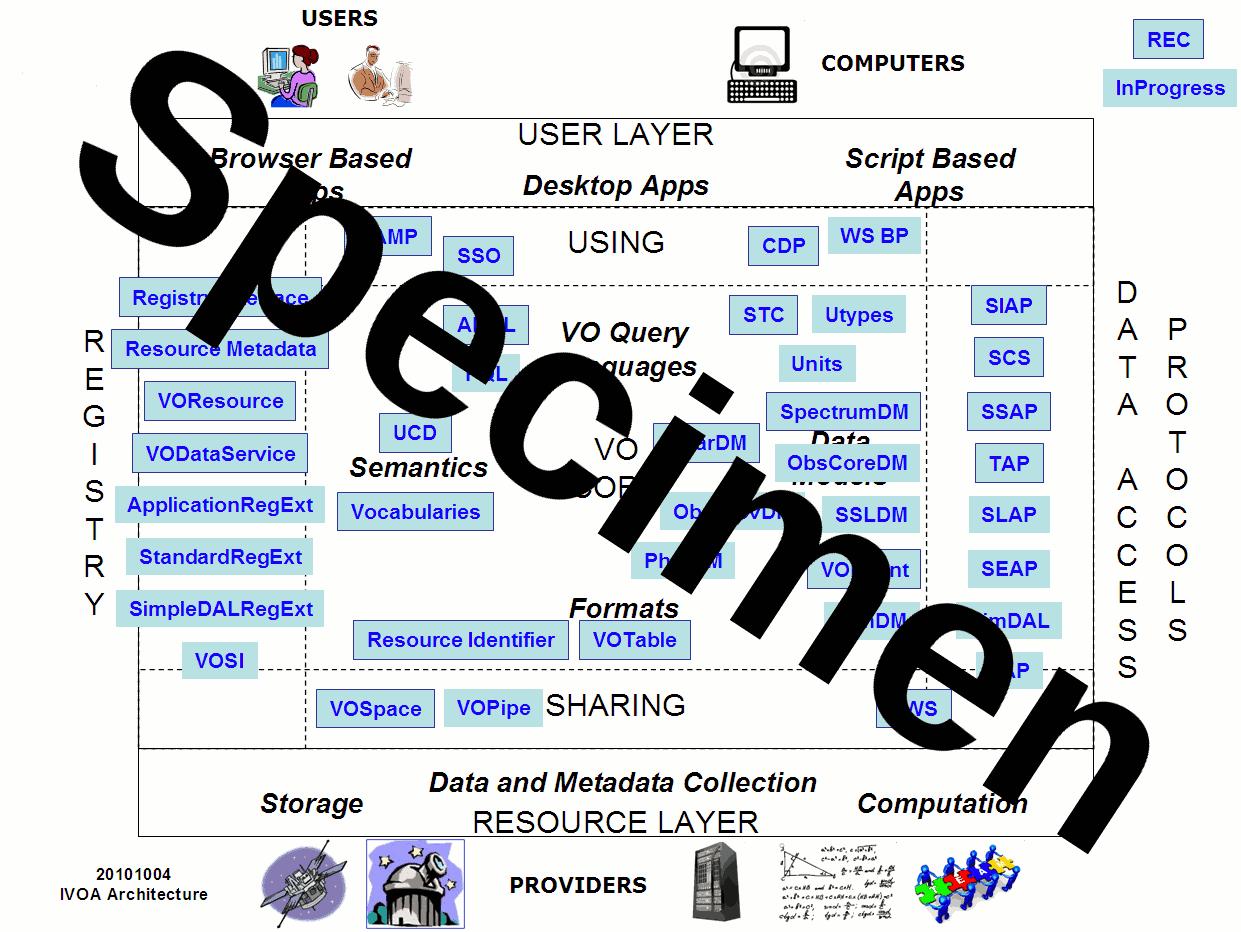
\includegraphics[width=0.9\textwidth]{archdiag.png}
\caption{Architecture diagram for this document}
\label{fig:archdiag}
\end{figure}

Fig.~\ref{fig:archdiag} shows the VOResource plays within the
IVOA architecture \citep{note:VOARCH}.

VOResource depends on the following other IVOA standards:

\begin{description}
\item[Resource Metadata, v1.12 \citep{2007ivoa.spec.0302H}] The RM
provides the central concepts and structures mapped here into an XML
schema.
\end{description}


There are relationships to the following other IVOA standards:

\begin{description}
\item[Registry Interfaces \citep{2009ivoa.spec.1104B}] Registry
Interfaces describes how registries exchange VOResource records, and it
provides a \xmlel{vr:Resource}-typed element to hold them within XML
data (VOResource itself has no global element).
\item[VOResource extensions] VOResource lays the foundations upon which
description schemes for concrete resources are built in various
VOResource extensions.  At the time of writing, recommendations have
been passed for the description of VO Standards
\citep{2012ivoa.spec.0508H}, various ``simple'' data discovery protocols
\citep{2013ivoa.spec.1125P}, generic data services
\citep{2010ivoa.spec.1202P}, and TAP services
\citep{2012ivoa.spec.0827D}.  The Registry Interfaces standard also
contains a VOResource extension.
\item[RegTAP \citep{2014ivoa.spec.1208D}] The Registry Relational Schema
gives a relational mapping of the models discussed here.
\item[VOSI \citep{2011ivoa.spec.0531G}] The VO support interfaces re-use
the service model developed here to facilitate service self-description.
\end{description}

\section{The VOResource Data Model}
\label{sect:model}

The primary use for VOResource, of course, is to describe a resource
using the metadata concepts defined in the RM.  Here is an example of a
VOResource document describing an organisation, the Radio Astronomy
Imaging Group at the National Center for Supercomputing Applications.  

\lstinputlisting[language=XML,numbers=right,basicstyle=\footnotesize]
   {example-voresource.xml}

This example illustrates some important components of a VOResource
record:

\begin{enumerate}
  \item the VOResource namespace (line 3),
  \item the specific type of resource indicated by
       the value of the \xmlel{xsi:type} attribute (line 2),
  \item the location of the schema documents used by
       this description (lines 5f) -- this is to facilitate document
       validation --,
  \item values for the three main types of core metadata:
       identity, curation, and content,
  \item a reference to another resource is made by
       providing that resource's IVOA identifier (line 13),
  \item string values can be padded with spaces
       for easier readability (e.g., line 17),
  \item extension metadata specific to the type of
       resource (lines 47ff).
\end{enumerate}


\subsection{The Schema Namespace and Location}

\label{sect:namespace}


The VOResource schema namespace is 
$$\hbox{\texttt{http://www.ivoa.net/xml/VOResource/v1.0}}.$$
The namespace URI has been chosen to allow it to be resolved as a URL
to the XML Schema document that defines the VOResource schema.
Applications may assume that the namespace URI is so resolvable.

Document authors are strongly encouraged to bind this namespace to the
\xmlel{vr:} prefix.  While in generic XML processing, the concrete
prefix used is irrelevant as long as the namespace URI mapped is the one
given by this specification, in the Virtual Observatory context uniform,
per-major-version prefixes are viewed as helping interoperability.  This
is particularly true when prefixes appear in attribute values (e.g.,
of \xmlel{xsi:type}), as non-schema aware XML processors cannot
URI-normalize such occurrences.  Also, non-XML-aware software (e.g., ADQL
engines) will use these prefixes rather than the full namespace URIs.

Authors of instance documents that use the VOResource schema may choose
to provide a location for VOResource XML Schema document using the
\xmlel{xsi:schemaLocation} attribute; the choice of the location value
is the choice of the author.  In general, the use of
\xmlel{xsi:schemaLocation} is recommended by this specification with
a the namespace URI given as the location as illustrated in the example
above, unless the application prefers otherwise.


\begin{verbatim}
xsi:schemaLocation="http://www.ivoa.net/xml/VOResource/v1.0
                    http://www.ivoa.net/xml/VOResource/v1.0"
\end{verbatim}

Because the VOResource XML schema sets \xmlel{elementFormDefault} to
unqualified, documents that use the VOResource schema must not bind the
empty namespace (using \verb|xmlns="..."|), anywhere in the document
where the VOResource schema is in effect.  This is a restriction set by
the rules of XML Schema.  Furthermore, in accordance with the Schema
rules for unqualified elements, the VOResource namespace prefix must not
used to qualify VOResource elements.  In general, namespace prefixes are
only used to qualify type names given as values to the \xmlel{xsi:type}
attribute (see next section).  Legal extensions of the VOResource schema
should also set \verb|elementFormDefault="unqualified"| for consistancy.



\subsection{The Core Structural and Semantic Model}
\label{sect:core}

The VOResource schema only defines global types; it does not define
any global elements (often referred to as root elements).  It is the
responsibility of the application to define the root element of the
VOResource-employing documents it operates on.  Typically, the root
element is defined in a separate application-specific schema.  The
type of an application document's root element is not assumed to be
any particular type defined in the VOResource schema (nor any of its
legal extensions).  In fact, it need not be of a type from the
VOResource at all; rather, VOResource types may appear anywhere in the
document.   

The IVOA Registry Interface standard \citep{2009ivoa.spec.1104B}, 
for example, at the time of writing includes a small schema that defines
a global element \xmlel{ri:Resource} of base type
\xmlel{vr:Resource}.  It is primarily intended as the child of
\xmlel{oai:metadata} in OAI-PMH responses \citep{std:oaipmh}, a protocol
frequently used to transport VOResource records.  When describing actual
resources, \xmlel{ri:Resource} will still use \xmlel{xsi:type} to
indicate the actual resource type.

Applications describe a single resource using an element of the type
\xmlel{vr:Resource} or a legal derivation of it.  The content of the
\xmlel{vr:Resource} type is referred to as the \textbf{core VOResource
metadata}, and they fall into four categories (corresponding to the
sections 3.1, 3.2, 3.3, and 4 of the RM):

\begin{itemize}
  \item identity metadata:  the \xmlel{title},
       \xmlel{shortName}, and
       \xmlel{identifier} elements;
  \item curation metadata:  the contents of the
       \xmlel{curation} element;
  \item general content metadata:  the contents of the
       \xmlel{content} element;
  \item metadata quality flags:  the
       \xmlel{validationLevel} element.
\end{itemize}


These elements are defined in more detail in sect.~\ref{sect:metadata}.


\begin{admonition}{Note}
In the example instance
document at the beginning of section~\ref{sect:model}, the root element,
\xmlel{resource} is not defined in any schema.
Nevertheless, this document is still legal and verifiable XML.
This is because the element's type is explicitly specified with
the \xmlel{xsi:type} attribute.
\end{admonition}


\subsubsection{Naming Convention}

VOResource uses the following conventions for
names of elements and types:

\begin{itemize}
  \item all global types it defines have names that are capitalized.
       (This practice would extend to global elements, if they existed
       in the VOResource.)   
  \item Locally defined elements begin with a lower-case character. 
  \item For all types and element names that are made up of multiple
       words, such as \xmlel{shortName}, upper-case letters are
       used demarcate the start of appended word (the ``camel''
       format).  
  \item Names that include abbreviations, such as
       \xmlel{IdentifierURI}, all letters in the abbreviation are
       capitalized.  
\end{itemize}

It is recommended that this convention be followed in other schemas
that either use the VOResource schema (via an \xmlel{xsd:import} or
\xmlel{xsd:include}) or extend it.  


\subsubsection{String Values}

Many of the elements in VOResource that are meant to have string or
URI values are defined as being of the type \xmlel{xs:token}.
This allows authors of VOResource instance documents to pad string and
URI values with spaces and include carriage returns to improve
readability.  The definition of these types will cause an XML
Schema-compliant parser to replace tab, line feed, and carriage return
characters with simple spaces, then replace multiple sequential
occurrences of spaces with a single space, and then remove all leading
and trailing spaces.

The \xmlel{description} children of resources and capabilities, on the
other hand, are of type \xmlel{xs:string}, which means that even
schema-aware processors will preserve whitespace.  This is inteded to
allow simple markup like paragraphs (empty lines) in the descriptions,
which may be little texts.  Since in VO practice, constructs like simple
ASCII tables sometimes appear in such descriptions, clients are
encouraged to not reflow descriptions and display them in a fixed-with
font.

\subsubsection{Language and Transliteration}

Several VOResource elements contain natural language (e.g.,
\xmlel{description}, \xmlel{title}, \xmlel{subject}).  In order to
ensure reliable discovery, in core VOResource, these elements must
contain English text, with US spelling strongly preferred; technically,
an \xmlel{xml:lang} value of \texttt{en-US} is implied.

Registry extensions may allow \xmlel{xml:lang} attributes on elements.
If they do, such elements must be repeatable, and an element without
\xmlel{xml:lang} (and hence, \texttt{en-US} implied) should be required
for global discoverability.  The requirements on \xmlel{xml:lang} from
the XML specification \citep{std:XML} apply.  Additionally, in
VOResource documents RFC 3066 language identifiers must be written in
lowercase.

Several VOResource elements contain names.  Again, for reliable global
discoverability, such names must be given in (common) English
transliteration where their original form uses non-Latin scripts.
Latin letters with diacritics are allowed, but Registry components are
generally expected to treat them equivalent to their base letters.

\subsubsection{Dates and Times}

All VOResource elements and attributes that contain dates must be
interpreted as UTC dates and must be encoded in compliance with ISO8601
\citep{std:iso8601}
standard Date and Time Format.  The \xmlel{vr:UTCTimestamp} type
provides a special restriction of the format that requires inclusion of
date and time, but enforces the use of the UTC timezone.  The time
format to be used by VOResource (designed to coincide with
what the OAI-PMH transport protocol mentioned above defines)
therefore requires timestamps like
$$\hbox{\texttt{2008-02-22T12:22:34Z,}}$$
where optional fractional seconds are allowed.  See the schema
documentation for the actual regular expression pattern.

For historical reasons, VOResource also allows a form without any
timezone marker.  Such timestamps are to be interpreted as  if they had
a trailing Z.

% GENERATED: !schemadoc VOResource-v1.1.xsd UTCTimestamp
\begin{generated}
\begingroup
      	\renewcommand*\descriptionlabel[1]{%
      	\hbox to 5.5em{\emph{#1}\hfil}}\vspace{2ex}\noindent\textbf{\xmlel{vr:UTCTimestamp} Type Schema Documentation}

\noindent{\small
           A timestamp that is compliant with ISO8601 and fixes
           the timezone indicator, if present, to "Z" (UTC).  VOResource
           writers should always include the timezone marker.  VOResource
           readers must interpret timestamps without a timezone marker as
           UTC.
         \par}

\vspace{1ex}\noindent\textbf{\xmlel{vr:UTCTimestamp} Type Schema Definition}

\begin{lstlisting}[language=XML,basicstyle=\footnotesize]
<xs:simpleType name="UTCTimestamp" >
  <xs:restriction base="xs:dateTime" >
    <xs:pattern
              value="\d{4}-\d\d-\d\dT\d\d:\d\d:\d\d(\.\d+)?Z?" />
  </xs:restriction>
</xs:simpleType>
\end{lstlisting}\endgroup
\end{generated}

% /GENERATED


Where day granularity might suffice, VOResource and extensions can
employ the \xmlel{vr:UTCDateTime} type.

% GENERATED: !schemadoc VOResource-v1.1.xsd UTCDateTime
\begin{generated}
\begingroup
      	\renewcommand*\descriptionlabel[1]{%
      	\hbox to 5.5em{\emph{#1}\hfil}}\vspace{2ex}\noindent\textbf{\xmlel{vr:UTCDateTime} Type Schema Documentation}

\noindent{\small
           A date stamp that can be given to a precision of either a
           day (type xs:date) or seconds (type xs:dateTime).  Where only a
           date is given, it is to be interpreted as the span of the day 
           on the UTC timezone if such distinctions are relevant.
         \par}

\vspace{1ex}\noindent\textbf{\xmlel{vr:UTCDateTime} Type Schema Definition}

\begin{lstlisting}[language=XML,basicstyle=\footnotesize]
<xs:simpleType name="UTCDateTime" >
  <xs:union memberTypes="xs:date vr:UTCTimestamp" />
</xs:simpleType>
\end{lstlisting}\endgroup
\end{generated}

% /GENERATED

\subsubsection{VOResource Semantics}

All VOResource types and elements have an associated semantic meaning
which is given in the first \xmlel{xsd:documentation}
node within the type or element's definition in the schema.  The
meaning associated with a type is generic, indicating the kind of
information the type provides.  The semantics that are delivered by a
VOResource instance document, however, are those associated with
VOResource elements.  The meaning of a VOResource element can be
thought of as having two parts:  the generic meaning of the set of
information it contains as defined by its type, and a specific meaning
describing the context in which that information applies.  Because all
VOResource elements are locally defined (in the XML Schema
sense), they do not have an absolute meaning, but rather have a
meaning tied to the thing being described by that element as
represented by the enclosing type.  

Here are three examples that illustrate the semantics communicated by
VOResource entities:

\begin{enumerate}
\item The \xmlel{vr:Curation} type describes the curation of a
       resource.  The \xmlel{curation} element
       describes curation of the specific resource described by the
       enclosing \xmlel{vr:Resource} type and identified by its
       \xmlel{identifier} element. 

  \item The \xmlel{vr:ResourceName} type is a generic reference to
       another resource.  The \xmlel{publisher} element
       gives a reference to the publisher of the specific resource being
       described which may itself be a registered resource described
       elsewhere.  

  \item The \xmlel{title} element gives the title of
       the resource being described by the enclosing
       \xmlel{vr:Resource} type and identified by its
       \xmlel{identifier} element.  The
       \xmlel{title} element's type,
       \xmlel{xs:token} (a restriction on
       \xmlel{xsd:string}), has no inherent meaning associated
       with it.   
\end{enumerate}


Additional semantics are transmitted through the use of derived types
using the \xmlel{xsi:type} attribute.  In the sample instance document
above, the use of \verb|xsi:type="vr:Organisation"| means that the
resource being described is specifically an organisation as defined by
the \xmlel{vr:Organisation} type.  This type provides additional
metadata that are not part of the core resource metadata.  The semantics
associated with the use of \xmlel{xsi:type} is described further in the
next subsection.



\subsubsection{Refined Semantics with Derived Types}
\label{sect:derivedtypes}

When a resource is described with an element explicitly of the type
\xmlel{vr:Resource}, it is being described in the most generic
sense.  The metadata presented in this type, including both free text
values and controlled vocabulary, can give some sense of what
type of resource is being described and what it might be used for.
However, the most useful descriptions of resources will not explicitly
use the \xmlel{vr:Resource} type; rather, they will use types
that are derived from \xmlel{vr:Resource}.  



Defining derived \xmlel{vr:Resource} types accomplishes two
things:
\begin{enumerate}
  \item it sharpens the semantic meaning of the resource description by
       indicating what specific type of resource it is, and
  \item it \emph{may} allow additional metadata not part of the core
       but specific to the that type of resource.
\end{enumerate}



The VOResource schema defines two types derived from
\xmlel{vr:Resource}:  \xmlel{vr:Organisation} and
\xmlel{vr:Service}.   The \xmlel{vr:Organisation} adds
metadata describing the astronomical facilities such as telescopes
that are associated with the organisation it describes.  The
\xmlel{vr:Service} type adds an element called
\xmlel{capability} which describes the service's interface as
well as information regarding its behavior.  



Extensions of the \xmlel{vr:Resource} type is a key way
derivation is used in VOResource to provide refined resource
descriptions.  Two other important parent types in the schema are
\xmlel{vr:Capability} and \xmlel{vr:Interface}; these are
extended to provide more refined descriptions of services (see
sect.~\ref{sect:servicemodel}).  The motivation for extending
these types is the same as for \xmlel{vr:Resource}: to provide
more specific semantic meaning through the derived type's name, and to
provide additional, specialized metadata that is not part of the
parent type.  Note, however, that in general, a derived type need not
alter the content model of its base type.  This allows derived types
to add more specific meaning with out adding any additional metadata.



As described in sect.~\ref{sect:core}, it is intended that derived
\xmlel{vr:Resource}, \xmlel{vr:Capability} and \xmlel{vr:Interface}
types be invoked in instance documents using the \xmlel{xsi:type}
attribute (as illustrated in the sample document above).  This method
illustrates a polymorphism for resource metadata in that any place where
an element of parent type is expected, the derived type may be inserted.
The use of \xmlel{xsi:type} illustrates both what specific type is being
inserted in as well as what it is being inserted in for.  That is, as in
our example, the \emph{resource} being described is an
\emph{organisation}.  



The other mechanism for polymorphism provided by XML Schema is
substitution groups.  Invoking derived \xmlel{vr:Resource} types via
elements in a substitution group is discouraged because it is less
obvious from looking at the instance document that a substitution is
being made.  


\subsubsection{The Service Data Model}
\label{sect:servicemodel}


The \xmlel{vr:Service} type extends the core \xmlel{vr:Resource}
metadata data by adding the \xmlel{capability} element (see
sect.~\ref{sect:serviceelements}).  This element is used to describe a major
functionality of the service, usually accessible through a single
service endpoint URL.  In particular, it is used to describe support for
an IVOA service standard (e.g. Simple Image Access Protocol).  A service
resource record may have multiple child \xmlel{capability} elements,
each describing a different major functionality; however, these
capabilities should be related in an obvious, logical way by virtue of
sharing the same core VOResource metadata.  


\begin{admonition}{Note}
Whether multiple related capabilities are grouped together in a
single Service record or are described in separate Service
records is expected to be the choice of the VOResource record
author.  However, it is also expected that resource registry
providers will provide some guidance to authors on best
practices.  This guidance could in part come in the form of a
GUI that naturally encourage or constrain aggregation of
capabilities in a single record.
\end{admonition}

The \xmlel{capability} element, through its type \xmlel{vr:Capability},
describes the behavior of service capability and how to access it.  The
latter is described by a child \xmlel{interface} element.  As for the
behavior, the base \xmlel{vr:Capability} type only provides a
\xmlel{description} element that can contain human-readable text on what
this capability provides.  More structured behavioral information must
be provided through specialized \xmlel{vr:Capability} extensions.  In
particular, a service standard (e.g. Simple Image
Access Protocol) will define an extension of \xmlel{vr:Capability} that
adds additional metadata that can describe the service's behavior in
relation to the standard (in practice, the Registry extension is
frequently defined in an separate ancillary standard). 

The added metadata can describe
limitations of the service implementation or indicate support for
optional features.  The specific \xmlel{vr:Capability} type is invoked
using the \xmlel{xsi:type} mechanism described in
sect.~\ref{sect:namespace}.


Here is an example for assigning a specialized Capability type for
a standard service capability.  In this example, it is assumed that
\xmlel{ExampleCapType} extension type is defined in a separate
schema document, the target namespace of which as been bound to the
\xmlel{ex:} prefix:
.
\begin{lstlisting}[language=XML]
<capability xsi:type="ex:ExampleCapType"
            standardID="ivo://example.com/std/exampleAccess">
  ...
</capability>
\end{lstlisting}

Note that the \xmlel{xsi:type} and the \xmlel{standardID} can vary
independently of each other.  There is no requirement to use a given
capability type for an endpoint conforming to a certain standard, as
indicated by the capability's \xmlel{standardID}. Conversely,
it may make sense to re-use a certain capability type in a different
standard; historically, several VOResource extension types have
fixed \xmlel{standardID}s.  This is now discouraged, as it needlessly
limits the applicability of the encoded metadata models.

If the service capability being described does not conform to any
standard or if the standard does not require any specialized
capability metadata for describing an implementation's behavior, then
\xmlel{vr:Capability} can be used as-is, possibly with the appropriate
\xmlel{standardID}.


Each \xmlel{capability} element can contain one or more child
\xmlel{interface} elements, each describing how the capability
can be accessed.  The \xmlel{interface} element's type,
\xmlel{vr:Interface}, is abstract; thus, the
\xmlel{interface} element must be accompanied by an
\xmlel{xsi:type} attribute that indicates an
\xmlel{vr:Interface} extension type.  The VOResource schema
defines two \xmlel{vr:Interface} extension types:
\xmlel{vr:WebBrowser}, for describing an interface access via web
browser, and \xmlel{vr:WebService}, for accessing a service
described by a Web Service Description Language (WSDL) document.


When a \xmlel{capability} contains more than one
\xmlel{interface}, each \xmlel{interface} should be
interpreted as an alternative interface for accessing essentially the
same underlying capability.  The interfaces can differ in their
overall type (e.g. \xmlel{vr:WebBrowser},
\xmlel{vr:WebService}) or in the supported input parameters or
output products.  


When a standard capability is being described (by means of providing a
\xmlel{standardID}), then at least one of the
\xmlel{interface} elements should describe an interface required
by the standard.  The \xmlel{role} attribute is used to mark the
standard interfaces (typically with the value ``std'').
All other interfaces are considered non-standard
alternatives.  To best support real-world discovery strategies, it is
recommended to avoid having non-standard interfaces in capabilities
with well-known \xmlel{standardID}s with the exception of
\xmlel{vr:WebBrowser}-typed ones.


Another way \xmlel{interface}s inside the same
\xmlel{capability} element can be used is if a standard forsees
different versions of a protocol within the same capability.  Different
interfaces can then be distinguished by different values of the
interface's \xmlel{version} attribute.  Previous versions of this
document in effect recommended this pattern for VO standards.

While this pattern can still be employed, most VO standards that
actually have different versions distinguish their endpoints by
different standard identifiers, as described in section 4.2 of IVOA
Identifiers 2.0 \citep{std:identifiers2}.  In these cases -- where the
\xmlel{capability}'s \xmlel{standardID} attribute already uniquely
determines the protocol spoken --, the specification of \xmlel{version}
on \xmlel{interface} elements is optional, though encouraged.

\subsection{Extending the VOResource Schema}

\label{sect:extending}

A schema made up only of global type definitions provides great
flexibility for extension.  Any global type defined in the VOResource
schema may be used as the base of a derived type defined in another
schema.  The schema containing the derived types must declare its own
namespace URI or default to the null namespace; it must not adopt the
VOResource namespace URI.  The application must then define what
schemas, identified by their namespace URIs, are supported and/or
required.  



A \textbf{VOResource extension} is an XML Schema document whose primary
purpose is to define new types derived from those defined in the
VOResource schema for use in resource descriptions.  It is recommended
that VOResource extensions follow the definition styles used by the core
VOResource.  In particular: 

\begin{itemize}
  \item \emph{Provide semantic definitions of all types and elements within
       the first \xmlel{xsd:documentation} element inside
       the type or element definition.}  Subsequent
       \xmlel{xsd:documentation} elements may provide
       additional comments or discussion.  

  \item \emph{Avoid the use of \xmlel{xsd:choice} elements.}
       VOResource does not use the choice structure because it does
       not map readily into any object-oriented software language
       structure.  Choices are handled instead as multiple derived
       types that can be inserted in place of a parent type.  

  \item \emph{Avoid the use of substitution groups}.  VOResource
       prefers instead the use of \xmlel{xsi:type} which are
       (with a few exceptions) functionally equivalent to substitution
       groups in terms of structure; however, \xmlel{xsi:type}
       serves as an obvious flag in the instance document that a
       substitution has been made. 

  \item \emph{Choose semantically meaningful names for derived
       types.}  When the derived type appears in the pattern
       \verb|<elname xsi:type="derivedType">|,
       choose a \textit{derivedType} name such that the sentence, ``a
       \textit{derivedType} is a kind of \textit{elname}'' makes natural
       and obvious sense.  For example, ``an \textit{Organisation} is a
       kind of \textit{resource}.'' 

  \item \emph{Follow the VOResource naming conventions}. 
\end{itemize}



There are two types of derivation that are particularly important to
the VOResource data model:  derivation of the \xmlel{vr:Resource}
type, used to define specific types of resources, and the derivation
of service metadata elements.  


\subsubsection{Defining New Resource Types}
\label{sect:definingresourcetypes}


Derivation of \xmlel{vr:Resource} to define new kinds of
resources should be done by extension (i.e. using 
\xmlel{xsd:extension}) rather than restriction.  It is
not required that the derived type change the content model from that
of the \xmlel{vr:Resource} base type; in this case, the purpose
of the derivation is only to sharpen the semantic meaning of the
resource description.  


\subsubsection{Defining New Service Capabilities and Interfaces}
\label{sect:serviceelements}


As described in sect.~\ref{sect:servicemodel}, a service
standard will often define a new \xmlel{vr:Capability} extension
type to allow implementations to describe how they support the
standard.  This definition of the \xmlel{vr:Capability} extension
should be done in a schema document with a namespace identifier that
is dedicated to that standard (hereafter referred to as \emph{the
standard's extension schema}).  The extension type should include
elements representing the applicable Capability metadata described in
section 5.2 of the RM
(e.g. \emph{Service.MaxReturnRecords}, \emph{Service.MaxReturnSize})
but can also include other concepts that are specific to that standard.


An extension schema can define new interface types, though not
necessarily in the context of any specific standard service
capability.  The basic \xmlel{vr:Interface} type provides only
\xmlel{accessURL}, \xmlel{mirrorURL}, and \xmlel{securityMethod} as child
elements.  A derived \xmlel{vr:Interface} type must indicate in
the documentation how the \xmlel{accessURL} should be
interpreted and used.  The derived type may also include other added
metadata describing how to use the service (e.g., a description of the
input arguments).  If the interface extension type is expected to be
referenced by a standard service capability, then it is recommended
that the additional metadata be optional unless the metadata is
absolutely required by clients in order to invoke the service.


Examples for extension schemas can be found in the IVOA Document
Repository.\footnote{\url{http://ivoa.net/documents}}
Sect.~\ref{sect:role} enumerates the ones in Recommendation state at the
time of writing.


\section{The VOResource Metadata}
\label{sect:metadata}


This section enumerates the types and elements defined in the
VOResource schema.


\subsection{The Base Resource Type}

\label{sect:restype}

A resource, as defined by the RM, is any entity or component of a VO
application that is describable and identifiable by a IVOA Identifier.
A resource is described using VOResource by an element of the type
\xmlel{vr:Resource} or one of its legal extensions.  The schema
definition (below) includes elements that encode the identity, curation,
and general content metadata for a resource (see sections 3.1 through
3.3 of the RM).  The RM states that certain metadata are required in a
minimally compliant resource description; this requirement is enforced
by the VOResource schema definition.  

% GENERATED: !schemadoc VOResource-v1.1.xsd Resource
\begin{generated}
\begingroup
      	\renewcommand*\descriptionlabel[1]{%
      	\hbox to 5.5em{\emph{#1}\hfil}}\vspace{2ex}\noindent\textbf{\xmlel{vr:Resource} Type Schema Documentation}

\noindent{\small
           Any entity or component of a VO application that is
           describable and identifiable by a IVOA Identifier. 
         \par}

\vspace{1ex}\noindent\textbf{\xmlel{vr:Resource} Type Schema Definition}

\begin{lstlisting}[language=XML,basicstyle=\footnotesize]
<xs:complexType name="Resource" >
  <xs:sequence >
    <xs:element name="validationLevel" type="vr:Validation" minOccurs="0"
              maxOccurs="unbounded" />
    <xs:element name="title" type="xs:token" />
    <xs:element name="shortName" type="vr:ShortName" minOccurs="0" />
    <xs:element name="identifier" type="vr:IdentifierURI" />
    <xs:element name="altIdentifier" type="xs:anyURI" minOccurs="0"
              maxOccurs="unbounded" />
    <xs:element name="curation" type="vr:Curation" />
    <xs:element name="content" type="vr:Content" />
  </xs:sequence>
  <xs:attribute name="created" type="xs:dateTime" use="required" />
  <xs:attribute name="updated" type="xs:dateTime" use="required" />
  <xs:attribute name="status" use="required" >
    <xs:simpleType >
      <xs:restriction base="xs:string" >
        <xs:enumeration value="active" />
        <xs:enumeration value="inactive" />
        <xs:enumeration value="deleted" />
      </xs:restriction>
    </xs:simpleType>
  </xs:attribute>
  <xs:attribute name="version" type="xs.token" />
</xs:complexType>
\end{lstlisting}

\vspace{0.5ex}\noindent\textbf{\xmlel{vr:Resource} Attributes}

\begingroup\small\begin{bigdescription}
\item[created]
\begin{description}
\item[Type] \xmlel{xs:dateTime}
\item[Meaning] 
              The UTC date and time this resource metadata description
              was created. 
            
\item[Occurrence] required
\item[Comment] 
              This timestamp must not be in the future.  This time is
              not required to be accurate; it should be at least
              accurate to the day.  Any insignificant time fields
              should be set to zero. 
            
\end{description}
\item[updated]
\begin{description}
\item[Type] \xmlel{xs:dateTime}
\item[Meaning] 
              The UTC date this resource metadata description was last updated.
            
\item[Occurrence] required
\item[Comment] 
              This timestamp must not be in the future.  This time is
              not required to be accurate; it should be at least
              accurate to the day.  Any insignificant time fields
              should be set to zero. 
            
\end{description}
\item[status]
\begin{description}
\item[Type] string with controlled vocabulary
\item[Meaning] 
              a tag indicating whether this resource is believed to be still
              actively maintained.
            
\item[Occurrence] required

\item[Allowed Values]\hfil
\begin{longtermsdescription}\item[active]
                      resource is believed to be currently maintained, and its
                      description is up to date (default). 
                   
\item[inactive]
                     resource is apparently not being maintained at the present.
                   
\item[deleted]
                      resource publisher has explicitly deleted the resource.
                   
\end{longtermsdescription}
\end{description}
\item[version]
\begin{description}
\item[Type] \xmlel{xs.token}
\item[Meaning] 
               The XML schema version for which this instance was written.
               Implementors should set this to the value of the version
               attribute of their schema's root (xs:schema) element.
               Clients may assume version 1.0 if this attribute is 
               missing.
            
\item[Occurrence] optional
\end{description}


\end{bigdescription}\endgroup



\vspace{0.5ex}\noindent\textbf{\xmlel{vr:Resource} Metadata Elements}

\begingroup\small\begin{bigdescription}\item[Element \xmlel{validationLevel}]
\begin{description}
\item[Type] \xmlel{vr:ValidationLevel} with optional attributes
\item[Meaning] 
                  A numeric grade describing the quality of the
                  resource description, when applicable, 
                  to be used to indicate the confidence an end-user
                  can put in the resource as part of a VO application
                  or research study. 
               
\item[Occurrence] optional; multiple occurrences allowed.
\item[Comment] 
                  See vr:ValidationLevel for an explanation of the
                  allowed levels.  
               
\item[Comment] 
                  Note that when this resource is a Service, this
                  grade applies to the core set of metadata.
                  Capability and interface metadata, as well as the
                  compliance of the service with the interface
                  standard, is rated by validationLevel tag in the 
                  capability element (see the vr:Service complex
                  type).  
               

\end{description}
\item[Element \xmlel{title}]
\begin{description}
\item[Type] string: \xmlel{xs:token}
\item[Meaning] 
                  the full name given to the resource
               
\item[Occurrence] required

\end{description}
\item[Element \xmlel{shortName}]
\begin{description}
\item[Type] string
\item[Meaning] 
                 A short name or abbreviation given to the resource.
               
\item[Occurrence] optional

\item[Comment] 
                 This name will be used where brief annotations for
                 the resource name are required.  Applications may 
                 use to refer to this resource in a compact display.   
               
\item[Comment] 
                 One word or a few letters is recommended.  No more
                 than sixteen characters are allowed.
               

\end{description}
\item[Element \xmlel{identifier}]
\begin{description}
\item[Type] an IVOA Identifier URI: vr:IdentifierURI
\item[Meaning] 
                 Unambiguous reference to the resource conforming to the IVOA
                 standard for identifiers
               
\item[Occurrence] required


\end{description}
\item[Element \xmlel{altIdentifier}]
\begin{description}
\item[Type] a URI: \xmlel{xs:anyURI}
\item[Meaning] 
                  A reference to this resource in a non-IVOA identifier
                  scheme, e.g., DOI or bibcode.  Always use the an URI scheme
                  here, e.g., doi:10.1016/j.epsl.2011.11.037.  For bibcodes,
                  use a form like bibcode:2008ivoa.spec.0222P.
               
\item[Occurrence] optional; multiple occurrences allowed.

\end{description}
\item[Element \xmlel{curation}]
\begin{description}
\item[Type] composite: \xmlel{vr:Curation}
\item[Meaning] 
               Information regarding the general curation of the resource
             
\item[Occurrence] required

\end{description}
\item[Element \xmlel{content}]
\begin{description}
\item[Type] composite: \xmlel{vr:Content}
\item[Meaning] 
               Information regarding the general content of the resource
             
\item[Occurrence] required

\end{description}


\end{bigdescription}\endgroup

\endgroup
\end{generated}

% /GENERATED

Note that the \xmlel{vr:Resource} attributes (\xmlel{created},
\xmlel{updated}, \xmlel{status}) represent a special class of
metadata: they describe the resource metadata description contained
within the \xmlel{vr:Resource} itself as opposed to the resource being
described.  Also note that with OAI-PMH 2.0, VOResource records that
would have a \xmlel{status} of \verb|deleted| should not occur since
OAI-PMH mandates that \xmlel{oai:metadata} is empty for deleted
records, and VOResource's \xmlel{status} essentially is a refinement of
OAI-PMH's \xmlel{status}.  Having VOResource records with \xmlel{status}
set to \verb|deleted| might still be useful outside of OAI-PMH.

The \xmlel{version} attribute of an \xmlel{vr:Resource} element gives
the version of the schema it was written against, as prescribed in the
IVOA Note ``XML Schema Versioning Policies''
\citep{note:schemaevolution}.  If missing, the value of this attribute
can be assumed to be 1.0.  This attribute should \emph{not} be used to
locate the schema file -- clients should either consult
\xmlel{schemaLocation} or retrieve the latest schema for the \xmlel{vr:}
namespace from the IVOA schema repository.

The following sections discuss the complex types mentioned in the above
definitions.
All rules and advice given in the ``Comments'' portions in
the RM definition for the individual items 
apply. In some details, in particular as regards enumerations of values,
this document deviates from RM in content.

\subsubsection{Identity Metadata}

The identity metadata described in the RM (section
3.1) are represented as top-level children of the
\xmlel{vr:Resource} type.

\todo{I think we should deprecate IdentifierURI (what's that URI in
there now?)  And then there'd be IVOID (which may have query parts and
fragments) and perhaps RegistryReference (as in ``Reference into the
registry'' with the current IdentifierURI's pattern.}
Two special types, \xmlel{vr:ShortName} and
\xmlel{vr:IdentifierURI} are defined to support identity
metadata.  The \xmlel{vr:ShortName} definition enforces the
16-character limit on shortNames.  

% GENERATED: !schemadoc VOResource-v1.1.xsd ShortName
\begin{generated}
\begingroup
      	\renewcommand*\descriptionlabel[1]{%
      	\hbox to 5.5em{\emph{#1}\hfil}}\vspace{2ex}\noindent\textbf{\xmlel{vr:ShortName} Type Schema Documentation}

\noindent{\small
         a short name or abbreviation given to something.
       \par}

\noindent{\small
         This name will be used where brief annotations for
         the resource name are required.  Applications may 
         use to refer to this resource in a compact display.   
       \par}

\noindent{\small
         One word or a few letters is recommended.  No more
         than sixteen characters are allowed.
       \par}

\vspace{1ex}\noindent\textbf{\xmlel{vr:ShortName} Type Schema Definition}

\begin{lstlisting}[language=XML,basicstyle=\footnotesize]
<xs:simpleType name="ShortName" >
  <xs:restriction base="xs:token" >
    <xs:maxLength value="16" />
  </xs:restriction>
</xs:simpleType>
\end{lstlisting}\endgroup
\end{generated}

% /GENERATED

% GENERATED: !schemadoc VOResource-v1.1.xsd IdentifierURI
\begin{generated}
\begingroup
      	\renewcommand*\descriptionlabel[1]{%
      	\hbox to 5.5em{\emph{#1}\hfil}}\vspace{2ex}\noindent\textbf{\xmlel{vr:IdentifierURI} Type Schema Documentation}

\noindent{\small
            A reference to a registry record.  Note that this is not
            suitable for some types of IVOA identifiers, as it does
            not admit query parts  or fragment identifiers.
         \par}

\vspace{1ex}\noindent\textbf{\xmlel{vr:IdentifierURI} Type Schema Definition}

\begin{lstlisting}[language=XML,basicstyle=\footnotesize]
<xs:simpleType name="IdentifierURI" >
  <xs:restriction base="xs:anyURI" >
    <xs:pattern
              value="ivo://[\w\d][\w\d\-_\.!~\*'\(\)\+=]{2,}(/[\w\d\-_\.!~\*'\(\)\+=]+(/[\w\d\-_\.!~\*'\(\)\+=]+)*)?" />
  </xs:restriction>
</xs:simpleType>
\end{lstlisting}\endgroup
\end{generated}

% /GENERATED



\subsubsection{Curation Metadata}


The curation metadata described in the RM (section
3.2) are bundled together into the \xmlel{vr:Resource} child element
\xmlel{curation}.  Its content is defined by the
\xmlel{vr:Curation} complex type.



% GENERATED: !schemadoc VOResource-v1.1.xsd Curation
\begin{generated}
\begingroup
      	\renewcommand*\descriptionlabel[1]{%
      	\hbox to 5.5em{\emph{#1}\hfil}}\vspace{2ex}\noindent\textbf{\xmlel{vr:Curation} Type Schema Documentation}

\noindent{\small
         Information regarding the general curation of a resource
       \par}

\vspace{1ex}\noindent\textbf{\xmlel{vr:Curation} Type Schema Definition}

\begin{lstlisting}[language=XML,basicstyle=\footnotesize]
<xs:complexType name="Curation" >
  <xs:sequence >
    <xs:element name="publisher" type="vr:ResourceName" />
    <xs:element name="creator" type="vr:Creator" minOccurs="0"
              maxOccurs="unbounded" />
    <xs:element name="contributor" type="vr:ResourceName" minOccurs="0"
              maxOccurs="unbounded" />
    <xs:element name="date" type="vr:Date" minOccurs="0"
              maxOccurs="unbounded" />
    <xs:element name="version" type="xs:token" minOccurs="0" />
    <xs:element name="contact" type="vr:Contact" maxOccurs="unbounded" />
  </xs:sequence>
</xs:complexType>
\end{lstlisting}

\vspace{0.5ex}\noindent\textbf{\xmlel{vr:Curation} Metadata Elements}

\begingroup\small\begin{bigdescription}\item[Element \xmlel{publisher}]
\begin{description}
\item[Type] string with ID attribute: vr:ResourceName
\item[Meaning] 
               Entity (e.g. person or organisation) responsible for making the 
               resource available
             
\item[Occurrence] required

\end{description}
\item[Element \xmlel{creator}]
\begin{description}
\item[Type] composite: \xmlel{vr:Creator}
\item[Meaning] 
                The entity (e.g. person or organisation) primarily responsible 
                for creating the content or constitution of the resource.
             
\item[Occurrence] optional; multiple occurrences allowed.
\item[Comment] 
                A logo need only be provided for the first occurrence.
                When multiple logos are supplied via multiple creator 
                elements, the application is free to choose which to
                use. 
             

\end{description}
\item[Element \xmlel{contributor}]
\begin{description}
\item[Type] string with ID attribute: vr:ResourceName
\item[Meaning] 
               Entity responsible for contributions to the content of
               the resource
             
\item[Occurrence] optional; multiple occurrences allowed.

\end{description}
\item[Element \xmlel{date}]
\begin{description}
\item[Type] \xmlel{vr:UTCDateTime} with optional attributes
\item[Meaning] 
               Date associated with an event in the life cycle of the
               resource.  
             
\item[Occurrence] optional; multiple occurrences allowed.
\item[Comment] 
               This will typically be associated with the creation or 
               availability (i.e., most recent release or version) of
               the resource.  Use the role attribute to clarify.
             

\end{description}
\item[Element \xmlel{version}]
\begin{description}
\item[Type] string: \xmlel{xs:token}
\item[Meaning] 
               Label associated with creation or availablilty of a version of 
               a resource.
             
\item[Occurrence] optional

\end{description}
\item[Element \xmlel{contact}]
\begin{description}
\item[Type] composite: \xmlel{vr:Contact}
\item[Meaning] 
               Information that can be used for contacting someone with
               regard to this resource.
             
\item[Occurrence] required; multiple occurrences allowed.

\end{description}


\end{bigdescription}\endgroup

\endgroup
\end{generated}

% /GENERATED

Several of the curation elements (most importantly,
\xmlel{publisher}\/) make use of the
\xmlel{vr:ResourceName} type.  This type provides a means of
referring to another resource both by name and by its IVOA
identifier.  Not all resources referred to using this type will
necessarily be registered and, therefore, will have an identifier;
thus, the identifier (which is encoded as an attribute) is optional. 


% GENERATED: !schemadoc VOResource-v1.1.xsd ResourceName
\begin{generated}
\begingroup
      	\renewcommand*\descriptionlabel[1]{%
      	\hbox to 5.5em{\emph{#1}\hfil}}\vspace{2ex}\noindent\textbf{\xmlel{vr:ResourceName} Type Schema Documentation}

\noindent{\small
         The name of a potentially registered resource.  That is, the entity
         referred to may have an associated identifier.
       \par}

\vspace{1ex}\noindent\textbf{\xmlel{vr:ResourceName} Type Schema Definition}

\begin{lstlisting}[language=XML,basicstyle=\footnotesize]
<xs:complexType name="ResourceName" >
  <xs:simpleContent >
    <xs:extension base="xs:token" >
      <xs:attribute name="ivo-id" type="vr:IdentifierURI" />
    </xs:extension>
  </xs:simpleContent>
</xs:complexType>
\end{lstlisting}

\vspace{0.5ex}\noindent\textbf{\xmlel{vr:ResourceName} Attributes}

\begingroup\small\begin{bigdescription}
\item[ivo-id]
\begin{description}
\item[Type] an IVOA Identifier URI: vr:IdentifierURI
\item[Meaning] 
                The IVOA identifier for the resource referred to.
              
\item[Occurrence] optional

\end{description}


\end{bigdescription}\endgroup

\endgroup
\end{generated}

% /GENERATED


The \xmlel{creator} element is defined by the \xmlel{vr:Creator} complex
type which bundles together the RM metadata \emph{Creator} and
\emph{Creator.Logo}.



% GENERATED: !schemadoc VOResource-v1.1.xsd Creator
\begin{generated}
\begingroup
      	\renewcommand*\descriptionlabel[1]{%
      	\hbox to 5.5em{\emph{#1}\hfil}}\vspace{2ex}\noindent\textbf{\xmlel{vr:Creator} Type Schema Documentation}

\noindent{\small
            The entity (e.g. person or organisation) primarily responsible 
            for creating something
         \par}

\vspace{1ex}\noindent\textbf{\xmlel{vr:Creator} Type Schema Definition}

\begin{lstlisting}[language=XML,basicstyle=\footnotesize]
<xs:complexType name="Creator" >
  <xs:sequence >
    <xs:element name="name" type="vr:ResourceName" />
    <xs:element name="logo" type="xs:anyURI" minOccurs="0" />
    <xs:element name="altIdentifier" type="xs:anyURI" minOccurs="0"
              maxOccurs="unbounded" />
  </xs:sequence>
</xs:complexType>
\end{lstlisting}

\vspace{0.5ex}\noindent\textbf{\xmlel{vr:Creator} Metadata Elements}

\begingroup\small\begin{bigdescription}\item[Element \xmlel{name}]
\begin{description}
\item[Type] string with ID attribute: vr:ResourceName
\item[Meaning] 
                  the name or title of the creating person or organization
              
\item[Occurrence] required
\item[Comment] 
                  Users of the creation should use this name in
                  subsequent credits and acknowledgements.

                  This should be exactly one name, preferably last name
                  first (as in {"}van der Waals, Johannes Diderik{"}).
              

\end{description}
\item[Element \xmlel{logo}]
\begin{description}
\item[Type] a URI: \xmlel{xs:anyURI}
\item[Meaning] 
                URL pointing to a graphical logo, which may be used to help 
                identify the information source
              
\item[Occurrence] optional

\end{description}
\item[Element \xmlel{altIdentifier}]
\begin{description}
\item[Type] a URI: \xmlel{xs:anyURI}
\item[Meaning] 
                  A reference to this entitiy in a non-IVOA identifier
                  scheme, e.g., orcid.  Always use a URI form including
                  a scheme here.  For Orcid, use a pattern like
                  orcid:0000-0000-0000-000X.
               
\item[Occurrence] optional; multiple occurrences allowed.

\end{description}


\end{bigdescription}\endgroup

\endgroup
\end{generated}

% /GENERATED

The \xmlel{Creator}'s \xmlel{name} should contain exactly one name.
Since the creator name is what Registry users use when searching for
resources ``by author'', it should be set with care.  To make sensible
collation simple for clients, person names should be formatted last name
first wherever appropriate.

In collaborative efforts, multiple creator elements should be used, one
element per person or organization involved.

Examples for encouraged use of creator include:

\begin{lstlisting}[language=XML,basicstyle=\footnotesize]
  <creator>
    <name>van der Waals, Johannes Diderik</name>
  </creator>
  <creator>
    <name>de Vaucouleurs, G.</name>
  </creator>
  <creator>
    <name>Zhang Hailong</name>
  </creator>
  <creator>
    IVOA Registry Working Group
  </creator>
\end{lstlisting}

While the following uses of creator do not make a resource record
technically invalid, they are frowned upon:

\begin{lstlisting}[language=XML,basicstyle=\footnotesize]
  <creator>
    <!-- do not include multiple names in one name element -->
    <name>Mornilov, V.G., Polkov, I.M., Bakharov, A.I</name>
  </creator>
  <creator>
    <!-- Do not include functions or similar -->
    <name>PI: Ita Varajedini</name>
  </creator>
  <creator>
    <!-- Do not abuse creator for provenance, do not include markup -->
    <name>All data is downloaded from the &lt;a href=http:...</name>
  </creator>
\end{lstlisting}

The \xmlel{Date} element's type, \xmlel{vr:Date}, is an extension of the
\xmlel{UTCDateTime} type that adds an
optional attribute called \xmlel{role}.  

The purpose of the role attribute is to indicate what aspect of the
resource the date describes. This allows several \xmlel{date} elements to be
provided, each with a different role. The possible values for this
attribute are not controlled by the schema.  The IVOA, however, defines
an RDF vocabulary at
\url{http://www.ivoa.net/rdf/voresource/date_role} from
which the \xmlel{role} terms should be taken if at all possible.  At the
time or writing, the vocabulary consists of three old-style VOResource
1.0 terms and terms from the DataCite Metadata 3.1.

The vocabulary can evolve independently of this specification.
Applications can rely on the presence of the \textsl{Updated}
(deprecated VOResource 1.0 synonym: \textsl{update}) and
\textsl{Created} (deprecated VOResource 1.0 synonym: \textsl{creation})
terms.  Applications are not expected to support semantic relationships
between the terms (except for mapping the deprecated VOResource 1.0
terms to the modern DataCite Metadata ones).

% GENERATED: !schemadoc VOResource-v1.1.xsd Date
\begin{generated}
\begingroup
      	\renewcommand*\descriptionlabel[1]{%
      	\hbox to 5.5em{\emph{#1}\hfil}}\vspace{1ex}\noindent\textbf{\xmlel{vr:Date} Type Schema Definition}

\begin{lstlisting}[language=XML,basicstyle=\footnotesize]
<xs:complexType name="Date" >
  <xs:simpleContent >
    <xs:extension base="vr:UTCDateTime" >
      <xs:attribute name="role" type="xs:string" default="representative" />
    </xs:extension>
  </xs:simpleContent>
</xs:complexType>
\end{lstlisting}

\vspace{0.5ex}\noindent\textbf{\xmlel{vr:Date} Attributes}

\begingroup\small\begin{bigdescription}
\item[role]
\begin{description}
\item[Type] string: \xmlel{xs:string}
\item[Meaning] 
                 A string indicating what the date refers to.  
               
\item[Occurrence] optional
representative
\item[Comment] 
               	The value of role should be taken from the RDF vocabulary
               	http://www.ivoa.net/rdf/voresource/date\_role.
               	This includes the the traditional and deprecated strings
                {"}creation{"}, indicating the date that the resource 
                itself was created, and {"}update{"}, indicating when the
                resource was updated last, and the default value,
                {"}representative{"}, meaning the date is a rough 
                representation of the time coverage of the resource.
                The preferred terms from that vocabulary are the DataCite
                Metadata terms.   It is expected that the vocabulary will 
                be kept synchronous with the corresponding list of terms
                in the DataCite Metadata schema.
               
\item[Comment] 
                 Note that this date refers to the resource; dates describing
                 the metadata description of the resource are handled by
                 the {"}created{"} and {"}updated{"} attributes of the Resource 
                 element. 
               
\end{description}


\end{bigdescription}\endgroup

\endgroup
\end{generated}

% /GENERATED



The \xmlel{contact} element is defined by the
\xmlel{vr:Contact} type which bundles together several component
pieces of information, including the RM metadata \emph{Contact.Name}
and \emph{Contact.Email}.  



% GENERATED: !schemadoc VOResource-v1.1.xsd Contact
\begin{generated}
\begingroup
      	\renewcommand*\descriptionlabel[1]{%
      	\hbox to 5.5em{\emph{#1}\hfil}}\vspace{2ex}\noindent\textbf{\xmlel{vr:Contact} Type Schema Documentation}

\noindent{\small
          Information that can be used for contacting someone
        \par}

\vspace{1ex}\noindent\textbf{\xmlel{vr:Contact} Type Schema Definition}

\begin{lstlisting}[language=XML,basicstyle=\footnotesize]
<xs:complexType name="Contact" >
  <xs:sequence >
    <xs:element name="name" type="vr:ResourceName" />
    <xs:element name="address" type="xs:token" minOccurs="0" />
    <xs:element name="email" type="xs:token" minOccurs="0" />
    <xs:element name="telephone" type="xs:token" minOccurs="0" />
  </xs:sequence>
</xs:complexType>
\end{lstlisting}

\vspace{0.5ex}\noindent\textbf{\xmlel{vr:Contact} Metadata Elements}

\begingroup\small\begin{bigdescription}\item[Element \xmlel{name}]
\begin{description}
\item[Type] string with ID attribute: vr:ResourceName
\item[Meaning] 
                  the name or title of the contact person.
              
\item[Occurrence] required
\item[Comment] 
                  This can be a person's name, e.g. {"}John P. Jones{"} or
                  a group, {"}Archive Support Team{"}.
              

\end{description}
\item[Element \xmlel{address}]
\begin{description}
\item[Type] string: \xmlel{xs:token}
\item[Meaning] the contact mailing address
\item[Occurrence] optional
\item[Comment] 
                All components of the mailing address are given in one
                string, e.g. {"}3700 San Martin Drive, Baltimore, MD 21218 USA{"}.
              

\end{description}
\item[Element \xmlel{email}]
\begin{description}
\item[Type] string: \xmlel{xs:token}
\item[Meaning] the contact email address
\item[Occurrence] optional

\end{description}
\item[Element \xmlel{telephone}]
\begin{description}
\item[Type] string: \xmlel{xs:token}
\item[Meaning] the contact telephone number
\item[Occurrence] optional
\item[Comment] 
                Complete international dialing codes should be given, e.g.
                {"}+1-410-338-1234{"}.
              

\end{description}


\end{bigdescription}\endgroup

\endgroup
\end{generated}

% /GENERATED



\subsubsection{General Content Metadata}


The general content metadata described in the RM
(section 3.3) are bundled together into the \xmlel{vr:Resource}
child element \xmlel{content}.  Its content is
defined by the \xmlel{vr:Content} complex type.


% GENERATED: !schemadoc VOResource-v1.1.xsd Content
\begin{generated}
\begingroup
      	\renewcommand*\descriptionlabel[1]{%
      	\hbox to 5.5em{\emph{#1}\hfil}}\vspace{2ex}\noindent\textbf{\xmlel{vr:Content} Type Schema Documentation}

\noindent{\small
         Information regarding the general content of a resource
       \par}

\vspace{1ex}\noindent\textbf{\xmlel{vr:Content} Type Schema Definition}

\begin{lstlisting}[language=XML,basicstyle=\footnotesize]
<xs:complexType name="Content" >
  <xs:sequence >
    <xs:element name="subject" type="xs:token" maxOccurs="unbounded" />
    <xs:element name="description" type="xs:string" />
    <xs:element name="source" type="vr:Source" minOccurs="0" />
    <xs:element name="referenceURL" type="xs:anyURI" />
    <xs:element name="type" type="xs:token" minOccurs="0"
              maxOccurs="unbounded" />
    <xs:element name="contentLevel" type="xs:token" minOccurs="0"
              maxOccurs="unbounded" />
    <xs:element name="relationship" type="vr:Relationship" minOccurs="0"
              maxOccurs="unbounded" />
  </xs:sequence>
</xs:complexType>
\end{lstlisting}

\vspace{0.5ex}\noindent\textbf{\xmlel{vr:Content} Metadata Elements}

\begingroup\small\begin{bigdescription}\item[Element \xmlel{subject}]
\begin{description}
\item[Type] string: \xmlel{xs:token}
\item[Meaning] 
               a topic, object type, or other descriptive keywords 
               about the resource.  
             
\item[Occurrence] required; multiple occurrences allowed.
\item[Comment] 
               Terms for Subject should be drawn from the IAU Astronomy 
               Thesaurus (http://msowww.anu.edu.au/library/thesaurus/).
             

\end{description}
\item[Element \xmlel{description}]
\begin{description}
\item[Type] string: \xmlel{xs:string}
\item[Meaning] 
               An account of the nature of the resource
             
\item[Occurrence] required
\item[Comment] 
               The description may include but is not limited to an abstract, 
               table of contents, reference to a graphical representation of
               content or a free-text account of the content.
             

\end{description}
\item[Element \xmlel{source}]
\begin{description}
\item[Type] a string with optional attributes
\item[Meaning] 
                a bibliographic reference from which the present resource is 
                derived or extracted.  
             
\item[Occurrence] optional
\item[Comment] 
                This is intended to point to an article in the published 
                literature.  An ADS Bibcode is recommended as a value when 
                available.    
             

\end{description}
\item[Element \xmlel{referenceURL}]
\begin{description}
\item[Type] a URI: \xmlel{xs:anyURI}
\item[Meaning] 
                URL pointing to a human-readable document describing this 
                resource.   
             
\item[Occurrence] required

\end{description}
\item[Element \xmlel{type}]
\begin{description}
\item[Type] string: \xmlel{xs:token}
\item[Meaning] 
               Nature or genre of the content of the resource.  Values for
               type should be taken from a controlled vocabulary, available 
               in RDF form from
               http://www.ivoa.net/rdf/voresource/content\_type
             
\item[Occurrence] optional; multiple occurrences allowed.

\end{description}
\item[Element \xmlel{contentLevel}]
\begin{description}
\item[Type] string: \xmlel{xs:token}
\item[Meaning] 
                Description of the content level or intended audience.
                Values for contentLevel should be taken from a controlled
                vocabulary, available at
                http://www.ivoa.net/rdf/voresource/content\_level.
             
\item[Occurrence] optional; multiple occurrences allowed.

\end{description}
\item[Element \xmlel{relationship}]
\begin{description}
\item[Type] composite: \xmlel{vr:Relationship}
\item[Meaning] 
               a description of a relationship to another resource.  
             
\item[Occurrence] optional; multiple occurrences allowed.

\end{description}


\end{bigdescription}\endgroup

\endgroup
\end{generated}

% /GENERATED



The \xmlel{source} element's type,
\xmlel{vr:Source}, is an extension of the
\xmlel{xs:token} type that adds an optional attribute called
\xmlel{format}.  


% GENERATED: !schemadoc VOResource-v1.1.xsd Source
\begin{generated}
\begingroup
      	\renewcommand*\descriptionlabel[1]{%
      	\hbox to 5.5em{\emph{#1}\hfil}}\vspace{1ex}\noindent\textbf{\xmlel{vr:Source} Type Schema Definition}

\begin{lstlisting}[language=XML,basicstyle=\footnotesize]
<xs:complexType name="Source" >
  <xs:simpleContent >
    <xs:extension base="xs:token" >
      <xs:attribute name="format" type="xs:string" />
    </xs:extension>
  </xs:simpleContent>
</xs:complexType>
\end{lstlisting}

\vspace{0.5ex}\noindent\textbf{\xmlel{vr:Source} Attributes}

\begingroup\small\begin{bigdescription}
\item[format]
\begin{description}
\item[Type] string: \xmlel{xs:string}
\item[Meaning] 
                 The reference format.  Recognized values include {"}bibcode{"}, 
                 referring to a standard astronomical bibcode 
                 (http://cdsweb.u-strasbg.fr/simbad/refcode.html).  
               
\item[Occurrence] optional
\end{description}


\end{bigdescription}\endgroup

\endgroup
\end{generated}

% /GENERATED


The \xmlel{relationship} is defined by the
\xmlel{vr:Relationship} complex type which bundles together the
RM metadata \emph{Relationship} and
\emph{RelationshipID}.  

The nature of the relationship is given by relationshipType.  The values
of this are taken from a vocabulary that is available in RDF form at
\url{http://www.ivoa.net/rdf/voresource/relationshipType}.  This
vocabulary at the time of writing consists of 

\begin{itemize}
\item the terms from VOResource 1.0 (mirror-of, service-for, served-by,
derived-from, and related-to); these are guaranteed to remain within
VOResource 1.x
\item selected terms from the DataCite Metadata relationType enumeration.
\end{itemize}

The resulting mix of term styles might be considered an aesthetic defect
but will not be homogenized in VOResource 1.x so as to neither
needlessly override DataCite practices nor interfere with existing uses
of the VOResource terms.

With the exception of the five VOResource 1.0 terms, the vocabulary may
change without changes to the recommendation.

% GENERATED: !schemadoc VOResource-v1.1.xsd Relationship
\begin{generated}
\begingroup
      	\renewcommand*\descriptionlabel[1]{%
      	\hbox to 5.5em{\emph{#1}\hfil}}\vspace{2ex}\noindent\textbf{\xmlel{vr:Relationship} Type Schema Documentation}

\noindent{\small
           A description of the relationship between one resource and one or
           more other resources.
         \par}

\vspace{1ex}\noindent\textbf{\xmlel{vr:Relationship} Type Schema Definition}

\begin{lstlisting}[language=XML,basicstyle=\footnotesize]
<xs:complexType name="Relationship" >
  <xs:sequence >
    <xs:element name="relationshipType" type="xs:token" />
    <xs:element name="relatedResource" type="vr:ResourceName" minOccurs="1"
              maxOccurs="unbounded" />
  </xs:sequence>
</xs:complexType>
\end{lstlisting}

\vspace{0.5ex}\noindent\textbf{\xmlel{vr:Relationship} Metadata Elements}

\begingroup\small\begin{bigdescription}\item[Element \xmlel{relationshipType}]
\begin{description}
\item[Type] string: \xmlel{xs:token}
\item[Meaning] 
                  the named type of relationship
               
\item[Occurrence] required
\item[Comment] 
                 The value  of relationshipType should be taken from the RDF
                 vocabulary
                 http://www.ivoa.net/rdf/voresource/relationshipType.
               

\end{description}
\item[Element \xmlel{relatedResource}]
\begin{description}
\item[Type] string with ID attribute: vr:ResourceName
\item[Meaning] 
                  the name of resource that this resource is related to.
               
\item[Occurrence] required; multiple occurrences allowed.

\end{description}


\end{bigdescription}\endgroup

\endgroup
\end{generated}

% /GENERATED


\subsubsection{Resource Record Quality with validationLevel}



The RM's \emph{ResourceValidationLevel} is encoded in the VOResource
schema with the \xmlel{validationLevel} element, which can appear in
multiple places within a \xmlel{vr:Resource} type or sub-type.  It may
appear zero or more times as direct children of a \xmlel{vr:Resource}
type and/or, if the resource is a \xmlel{vr:Service} type or sub-type,
zero or more times as the first children of any \xmlel{capability}
element.  

The \xmlel{validationLevel} element requires an attribute called
\xmlel{validatedBy} which takes an IVOID as a value.  This IVOID
must refer to a registered organisation or registry that assigned the
numerical value.  This element can appear multiple times, each with
a different \xmlel{validatedBy} value, to reflect the code
assigned by different organisations. 


% GENERATED: !schemadoc VOResource-v1.1.xsd ValidationLevel
\begin{generated}
\begingroup
      	\renewcommand*\descriptionlabel[1]{%
      	\hbox to 5.5em{\emph{#1}\hfil}}\vspace{2ex}\noindent\textbf{\xmlel{vr:ValidationLevel} Type Schema Documentation}

\noindent{\small
         The allowed values for describing the resource descriptions
         and interfaces.  
       \par}

\noindent{\small
         See the RM (v1.1, section 4) for more guidance on the use of
         these values.  
       \par}

\vspace{2ex}\noindent\textbf{\xmlel{vr:ValidationLevel} Type Allowed Values}

\begin{longtermsdescription}\item[0]
              The resource has a description that is stored in a
              registry. This level does not imply a compliant
              description. 
            
\item[1]
              In addition to meeting the level 0 definition, the
              resource description conforms syntactically to this
              standard and to the encoding scheme used. 
            
\item[2]
              In addition to meeting the level 1 definition, the
              resource description refers to an existing resource that
              has demonstrated to be functionally compliant. 
            
\item[3]
              In addition to meeting the level 2 definition, the
              resource description has been inspected by a human and
              judged to comply semantically to this standard as well
              as meeting any additional minimum quality criteria (e.g.,
              providing values for important but non-required
              metadata) set by the human inspector.
            
\item[4]
              In addition to meeting the level 3 definition, the
              resource description meets additional quality criteria
              set by the human inspector and is therefore considered
              an excellent description of the resource. Consequently,
              the resource is expected to operate well as part of a
              VO application or research study.
            
\end{longtermsdescription}
\vspace{1ex}\noindent\textbf{\xmlel{vr:ValidationLevel} Type Schema Definition}

\begin{lstlisting}[language=XML,basicstyle=\footnotesize]
<xs:simpleType name="ValidationLevel" >
  <xs:restriction base="xs:integer" >
    <xs:whiteSpace value="collapse" />
    <xs:enumeration value="0" />
    <xs:enumeration value="1" />
    <xs:enumeration value="2" />
    <xs:enumeration value="3" />
    <xs:enumeration value="4" />
  </xs:restriction>
</xs:simpleType>
\end{lstlisting}\endgroup
\end{generated}

% /GENERATED

% GENERATED: !schemadoc VOResource-v1.1.xsd Validation
\begin{generated}
\begingroup
      	\renewcommand*\descriptionlabel[1]{%
      	\hbox to 5.5em{\emph{#1}\hfil}}\vspace{2ex}\noindent\textbf{\xmlel{vr:Validation} Type Schema Documentation}

\noindent{\small
         a validation stamp combining a validation level and the ID of 
         the validator.
       \par}

\vspace{1ex}\noindent\textbf{\xmlel{vr:Validation} Type Schema Definition}

\begin{lstlisting}[language=XML,basicstyle=\footnotesize]
<xs:complexType name="Validation" >
  <xs:simpleContent >
    <xs:extension base="vr:ValidationLevel" >
      <xs:attribute name="validatedBy" type="vr:IdentifierURI" use="required" />
    </xs:extension>
  </xs:simpleContent>
</xs:complexType>
\end{lstlisting}

\vspace{0.5ex}\noindent\textbf{\xmlel{vr:Validation} Attributes}

\begingroup\small\begin{bigdescription}
\item[validatedBy]
\begin{description}
\item[Type] an IVOA Identifier URI: vr:IdentifierURI
\item[Meaning] 
               The IVOA ID of the registry or organisation that
               assigned the validation level.  
             
\item[Occurrence] required

\end{description}


\end{bigdescription}\endgroup

\endgroup
\end{generated}

% /GENERATED

\subsection{Resource Type Extensions:  Organisation and Service}

The VOResource schema defines two extensions of the base
\xmlel{vr:Resource} type for describing two specific types of
resources:  \xmlel{vr:Organisation} and \xmlel{vr:Service}.  In
addition to providing more refined semantic meanings over
\xmlel{vr:Resource}, they add additional metadata for the
describing the resource which do not necessarily apply in the generic
case. 



\subsubsection{The Organisation Resource Type}


The \xmlel{vr:Organisation} resource type is used to describe an organisation in
the sense defined by the RM:


\begin{quotation}
An organisation is a specific type of resource that brings people
together to pursue participation in VO applications.  Organisations
can be hierarchical and range greatly in size and scope.  At a high
level, an organisation could be a university, observatory, or
government agency.  At a finer level, it could be a specific
scientific project space mission, or individual researcher.  
\end{quotation}


The Organisation type extends the Resource type by adding two additional
elements to the core set of metadata, \xmlel{facility} and
\xmlel{instrument}:


% GENERATED: !schemadoc VOResource-v1.1.xsd Organisation
\begin{generated}
\begingroup
      	\renewcommand*\descriptionlabel[1]{%
      	\hbox to 5.5em{\emph{#1}\hfil}}\vspace{2ex}\noindent\textbf{\xmlel{vr:Organisation} Type Schema Documentation}

\noindent{\small
           A named group of one or more persons brought together to pursue 
           participation in VO applications.  
         \par}

\noindent{\small
           According to the Resource Metadata Recommendation, organisations 
           "can be hierarchical and range in size and scope.  At a high level, 
           an organisation could be a university, observatory, or government
           agency.  At a finer level, it could be a specific scientific 
           project, mission, or individual researcher."  
         \par}

\noindent{\small
           The main purpose of an organisation as a registered resource is 
           to serve as a publisher of other resources.  
         \par}

\vspace{1ex}\noindent\textbf{\xmlel{vr:Organisation} Type Schema Definition}

\begin{lstlisting}[language=XML,basicstyle=\footnotesize]
<xs:complexType name="Organisation" >
  <xs:complexContent >
    <xs:extension base="vr:Resource" >
      <xs:sequence >
        <xs:element name="facility" type="vr:ResourceName" minOccurs="0"
                  maxOccurs="unbounded" />
        <xs:element name="instrument" type="vr:ResourceName" minOccurs="0"
                  maxOccurs="unbounded" />
      </xs:sequence>
    </xs:extension>
  </xs:complexContent>
</xs:complexType>
\end{lstlisting}

\vspace{0.5ex}\noindent\textbf{\xmlel{vr:Organisation} Extension Metadata Elements}

\begingroup\small\begin{bigdescription}\item[Element \xmlel{facility}]
\begin{description}
\item[Type] string with ID attribute: vr:ResourceName
\item[Meaning] 
                       the observatory or facility used to collect the data 
                       contained or managed by this resource.  
                     
\item[Occurrence] optional; multiple occurrences allowed.

\end{description}
\item[Element \xmlel{instrument}]
\begin{description}
\item[Type] string with ID attribute: vr:ResourceName
\item[Meaning] 
                       the Instrument used to collect the data contain or 
                       managed by a resource.  
                     
\item[Occurrence] optional; multiple occurrences allowed.

\end{description}


\end{bigdescription}\endgroup

\endgroup
\end{generated}

% /GENERATED

The main role of an organisation in the VO (that is, the main reason
for describing organisations in a registry) is as a provider or
publisher of other resources.  In particular, an organisation
description in a registry declares the association of an IVOA
identifier with the organisation.  The
organisation can then be referred to in other resource descriptions.
For example, an organisation identifier will appear as the publisher
identifier of service resource (as illustrated in the opening
example in sect.~\ref{sect:model}).


\subsubsection{The Service Resource Type}


The \xmlel{vr:Service} resource type is used to describe a service--a resource
that actually does something--in the sense defined by the
RM:

\begin{quotation}
A service is any VO resource that can be invoked by the user to
perform some action on their behalf.  
\end{quotation}


The general data model is described in sect.~\ref{sect:servicemodel}.
The Service type extends the Resource type by adding two elements:
\xmlel{rights} which indicates the modalities of service use and access, and
\xmlel{capability} which describes how the service behaves and how it is
invoked.


% GENERATED: !schemadoc VOResource-v1.1.xsd Service
\begin{generated}
\begingroup
      	\renewcommand*\descriptionlabel[1]{%
      	\hbox to 5.5em{\emph{#1}\hfil}}\vspace{2ex}\noindent\textbf{\xmlel{vr:Service} Type Schema Documentation}

\noindent{\small
           a resource that can be invoked by a client to perform some action
           on its behalf.  
         \par}

\vspace{1ex}\noindent\textbf{\xmlel{vr:Service} Type Schema Definition}

\begin{lstlisting}[language=XML,basicstyle=\footnotesize]
<xs:complexType name="Service" >
  <xs:complexContent >
    <xs:extension base="vr:Resource" >
      <xs:sequence >
        <xs:element name="rights" type="vr:Rights" minOccurs="0"
                  maxOccurs="unbounded" />
        <xs:element name="capability" type="vr:Capability" minOccurs="0"
                  maxOccurs="unbounded" />
      </xs:sequence>
    </xs:extension>
  </xs:complexContent>
</xs:complexType>
\end{lstlisting}

\vspace{0.5ex}\noindent\textbf{\xmlel{vr:Service} Extension Metadata Elements}

\begingroup\small\begin{bigdescription}\item[Element \xmlel{rights}]
\begin{description}
\item[Type] composite: \xmlel{vr:Rights}
\item[Meaning] 
                       Information about rights held in and over the resource.
                     
\item[Occurrence] optional; multiple occurrences allowed.
\item[Comment] 
                       This should be repeated for all Rights values that apply.
                     

\end{description}
\item[Element \xmlel{capability}]
\begin{description}
\item[Type] composite: \xmlel{vr:Capability}
\item[Meaning] 
                        a description of a general capability of the
                        service and how to use it.
                     
\item[Occurrence] optional; multiple occurrences allowed.
\item[Comment] 
                        This describes a general function of the
                        service, usually in terms of a standard
                        service protocol (e.g. SIA), but not
                        necessarily so.
                     
\item[Comment] 
                        A service can have many capabilities
                        associated with it, each reflecting different
                        aspects of the functionality it provides.  
                     

\end{description}


\end{bigdescription}\endgroup

\endgroup
\end{generated}

% /GENERATED

The \xmlel{rights} element contains free text, where it is recommended
that standard licenses are named and special circumstances like embargoes
are mentioned.  The \xmlel{rightsURI} attribute can be used to
reference the
full license text.  By re-using standard URIs (e.g., provided by the
creators of the licenses), machines can
identify usage conditions.


% GENERATED: !schemadoc VOResource-v1.1.xsd Rights
\begin{generated}
\begingroup
      	\renewcommand*\descriptionlabel[1]{%
      	\hbox to 5.5em{\emph{#1}\hfil}}\vspace{2ex}\noindent\textbf{\xmlel{vr:Rights} Type Schema Documentation}

\noindent{\small
            A statement of usage rights.  This will typically be a license,
            which should be given as a full string (e.g., Creative Commons
            Attribution 3.0 International).  Further free-text information,
            e.g., on how to attribute or on embargo periods is allowed.
         \par}

\vspace{1ex}\noindent\textbf{\xmlel{vr:Rights} Type Schema Definition}

\begin{lstlisting}[language=XML,basicstyle=\footnotesize]
<xs:complexType name="Rights" >
  <xs:complexContent >
    <xs:extension base="xs:token" >
      <xs:attribute name="rightsURI" type="xs:anyURI" />
    </xs:extension>
  </xs:complexContent>
</xs:complexType>
\end{lstlisting}

\vspace{0.5ex}\noindent\textbf{\xmlel{vr:Rights} Attributes}

\begingroup\small\begin{bigdescription}
\item[rightsURI]
\begin{description}
\item[Type] a URI: \xmlel{xs:anyURI}
\item[Meaning] 
                     A URI identifier for a license
                  
\item[Occurrence] optional
\item[Comment] 
                     Where formal licenses are available, this URI can
                     reference the full license text.  The IVOA may define
                     standard URIs (probably IVOIDs) for a set of recommended
                     licenses, in which case these should be used here.
                  
\end{description}


\end{bigdescription}\endgroup

\endgroup
\end{generated}

% /GENERATED

An example could look like this:

\begin{lstlisting}[language=XML,basicstyle=\footnotesize]
<rights rightsURI="http://creativecommons.org/licenses/by/3.0">
  The images from the X survey are copyright 2016, the X project.
  They are published under the creative commons attribution 3.0 unported
  license.  If you use this data, please cite doi:10.5072/7273288.

  Images are under embargo for one year after their addition to the
  repository.
</rights>
\end{lstlisting}

As described in sect.~\ref{sect:servicemodel}, multiple
\xmlel{capability} elements may appear, each describing a
different capability of the service.  


% GENERATED: !schemadoc VOResource-v1.1.xsd Capability
\begin{generated}
\begingroup
      	\renewcommand*\descriptionlabel[1]{%
      	\hbox to 5.5em{\emph{#1}\hfil}}\vspace{2ex}\noindent\textbf{\xmlel{vr:Capability} Type Schema Documentation}

\noindent{\small
            a description of what the service does (in terms of 
            context-specific behavior), and how to use it (in terms of
            an interface)
         \par}

\vspace{1ex}\noindent\textbf{\xmlel{vr:Capability} Type Schema Definition}

\begin{lstlisting}[language=XML,basicstyle=\footnotesize]
<xs:complexType name="Capability" >
  <xs:sequence >
    <xs:element name="validationLevel" type="vr:Validation" minOccurs="0"
              maxOccurs="unbounded" />
    <xs:element name="description" type="xs:string" minOccurs="0" />
    <xs:element name="interface" type="vr:Interface" minOccurs="0"
              maxOccurs="unbounded" />
  </xs:sequence>
  <xs:attribute name="standardID" type="xs:anyURI" />
</xs:complexType>
\end{lstlisting}

\vspace{0.5ex}\noindent\textbf{\xmlel{vr:Capability} Attributes}

\begingroup\small\begin{bigdescription}
\item[standardID]
\begin{description}
\item[Type] a URI: \xmlel{xs:anyURI}
\item[Meaning] 
               A URI identifier for a standard service. 
            
\item[Occurrence] optional
\item[Comment] 
               This provides a unique way to refer to a service
               specification standard, such as a Simple Image Access service.
               The use of an IVOA identifier here implies that a
               VOResource description of the standard is registered and 
               accessible.  
            
\end{description}


\end{bigdescription}\endgroup



\vspace{0.5ex}\noindent\textbf{\xmlel{vr:Capability} Metadata Elements}

\begingroup\small\begin{bigdescription}\item[Element \xmlel{validationLevel}]
\begin{description}
\item[Type] \xmlel{vr:ValidationLevel} with optional attributes
\item[Meaning] 
                  A numeric grade describing the quality of the
                  capability description and interface, when applicable, 
                  to be used to indicate the confidence an end-user
                  can put in the resource as part of a VO application
                  or research study. 
               
\item[Occurrence] optional; multiple occurrences allowed.
\item[Comment] 
                  See vr:ValidationLevel for an explanation of the
                  allowed levels.  
               

\end{description}
\item[Element \xmlel{description}]
\begin{description}
\item[Type] string: \xmlel{xs:string}
\item[Meaning] 
                  A human-readable description of what this capability 
                  provides as part of the over-all service 
               
\item[Occurrence] optional
\item[Comment] 
                  Use of this optional element is especially encouraged when
                  this capability is non-standard and is one of several 
                  capabilities listed.
               

\end{description}
\item[Element \xmlel{interface}]
\begin{description}
\item[Type] composite: \xmlel{vr:Interface}
\item[Meaning] 
                  a description of how to call the service to access
                  this capability
               
\item[Occurrence] optional; multiple occurrences allowed.
\item[Comment] 
                  Since the Interface type is abstract, one must describe
                  the interface using a subclass of Interface, denoting
                  it via xsi:type.
               
\item[Comment] 
                  Multiple occurences can describe different interfaces to 
                  the logically same capability--i.e. data or functionality.
                  That is, the inputs accepted and the output provides should
                  be logically the same.  For example, a WebBrowser interface
                  given in addition to a WebService interface would simply 
                  provide an interactive, human-targeted interface to the 
                  underlying WebService interface.  
               

\end{description}


\end{bigdescription}\endgroup

\endgroup
\end{generated}

% /GENERATED


The \xmlel{capability} element is sufficient for describing a
\emph{custom service capability}--i.e., a service that is
particular to one provider and does not conform to a specific standard 
(be it recognized by the IVOA or some other sub-community).  However,
service standards will often create a \xmlel{vr:Capability}
extension that adds additional metadata that are specific that that
are specific to the behavior of that particular type of service.  



\begin{admonition}{Note}
The RM defines three pieces of metadata that may be
important for several standard query services:
\emph{Service.MaxSearchRadius},
\emph{Service.MaxReturnRecords}, and
\emph{Service.MaxReturnSize}.  These are examples of
service-specific metadata that should be encoded as child
elements in a type derived from \xmlel{vr:Capability}.  
\end{admonition}


The \xmlel{interface} element is of the complex type 
\xmlel{vr:Interface}.

The \xmlel{vr:Interface} type is defined as abstract, so as described in
sect.~\ref{sect:servicemodel}, it must not be
used as part of a \xmlel{vr:Service} description unless it includes an
\xmlel{xsi:type} attribute that refers to a type derived from
\xmlel{vr:Interface}. The VOResource schema defines two derived
\xmlel{vr:Interface} types: \xmlel{vr:WebBrowser} and
\xmlel{vr:WebService}.

As described in sect.~\ref{sect:servicemodel}, the \xmlel{vr:Interface}
attributes help distinguish between multiple interfaces within the same
\xmlel{capability} element:


% GENERATED: !schemadoc VOResource-v1.1.xsd Interface
\begin{generated}
\begingroup
      	\renewcommand*\descriptionlabel[1]{%
      	\hbox to 5.5em{\emph{#1}\hfil}}\vspace{2ex}\noindent\textbf{\xmlel{vr:Interface} Type Schema Documentation}

\noindent{\small
            A description of a service interface.
         \par}

\noindent{\small
            Since this type is abstract, one must use an Interface subclass
            to describe an actual interface.
         \par}

\noindent{\small
           Additional interface subtypes (beyond WebService and WebBrowser) are 
           defined in the VODataService schema.
         \par}

\vspace{1ex}\noindent\textbf{\xmlel{vr:Interface} Type Schema Definition}

\begin{lstlisting}[language=XML,basicstyle=\footnotesize]
<xs:complexType name="Interface" abstract="true" >
  <xs:sequence >
    <xs:element name="accessURL" type="vr:AccessURL" minOccurs="1"
              maxOccurs="unbounded" />
    <xs:element name="mirrorURL" type="vr:MirrorURL" minOccurs="1"
              maxOccurs="unbounded" />
    <xs:element name="securityMethod" type="vr:SecurityMethod" minOccurs="0"
              maxOccurs="unbounded" />
    <xs:element name="testQueryString" type="xs:token" minOccurs="0"
              maxOccurs="unbounded" />
  </xs:sequence>
  <xs:attribute name="version" type="xs:string" />
  <xs:attribute name="role" type="xs:NMTOKEN" />
</xs:complexType>
\end{lstlisting}

\vspace{0.5ex}\noindent\textbf{\xmlel{vr:Interface} Attributes}

\begingroup\small\begin{bigdescription}
\item[version]
\begin{description}
\item[Type] string: \xmlel{xs:string}
\item[Meaning] 
               The version of a standard interface specification that this 
               interface complies with.  Most VO standards indicate the
               version in the standardID attribute of the capability.  For
               these standards, the version attribute should not be used.
            
\item[Occurrence] optional
\end{description}
\item[role]
\begin{description}
\item[Type] \xmlel{xs:NMTOKEN}
\item[Meaning] 
               A tag name the identifies the role the interface plays
               in the particular capability.  If the value is equal to
               {"}std{"} or begins with {"}std:{"}, then the interface refers
               to a standard interface defined by the standard
               referred to by the capability's standardID attribute.  
            
\item[Occurrence] optional
\item[Comment] 
               For an interface complying with some registered
               standard (i.e. has a legal standardID), the role can be
               match against interface roles enumerated in standard 
               resource record.  The interface descriptions in
               the standard record can provide default descriptions 
               so that such details need not be repeated here.  
            
\end{description}


\end{bigdescription}\endgroup



\vspace{0.5ex}\noindent\textbf{\xmlel{vr:Interface} Metadata Elements}

\begingroup\small\begin{bigdescription}\item[Element \xmlel{accessURL}]
\begin{description}
\item[Type] a URI with optional attributes
\item[Meaning] 
                 The URL (or base URL) that a client uses to access the
                 service.  How this URL is to be interpreted and used 
                 depends on the specific Interface subclass
               
\item[Occurrence] required; multiple occurrences allowed.
\item[Comment] 
                 Although the schema allows multiple occurrences of
                 accessURL, multiple accessURLs are deprecated.  Each
                 interface should have exactly one access URL.  Where an
                 interface has several mirrors, the  accessURL should
                 reflect the “primary” (fastest, best-connected, 
                 best-maintained) site, the one that non-sophisticated
                 clients will go to.

                 Additional accessURLs should be put into mirrorURLs.
                 Advanced clients can retrieve the mirrorURLs and 
                 empirically determine interfaces closer to their 
                 network location.
               

\end{description}
\item[Element \xmlel{mirrorURL}]
\begin{description}
\item[Type] a URI with optional attributes
\item[Meaning] 
                 A (base) URL of a mirror of this interface.  As with
                 accessURL, how this URL is to be interpreted and used 
                 depends on the specific Interface subclass
               
\item[Occurrence] required; multiple occurrences allowed.
\item[Comment] 
                This is intended exclusively for true mirrors, i.e.,
                interfaces that are functionally identical to the
                original interface and that are operated by the same 
                publisher.  Other arrangements should be represented as
                separate services linked by mirror-of relationships.
               

\end{description}
\item[Element \xmlel{securityMethod}]
\begin{description}
\item[Type] composite: \xmlel{vr:SecurityMethod}
\item[Meaning] 
                  the mechanism the client must employ to gain secure
                  access to the service.  
               
\item[Occurrence] optional; multiple occurrences allowed.
\item[Comment] 
                  when more than one method is listed, each one must
                  be employed to gain access.  
               

\end{description}
\item[Element \xmlel{testQueryString}]
\begin{description}
\item[Type] string: \xmlel{xs:token}
\item[Meaning] 
                  Test data for exercising the service.
               
\item[Occurrence] optional; multiple occurrences allowed.
\item[Comment] 
                  This contains data that can be passed to the interface to
                  retrieve a non-empty result.  This can be used by validators
                  within test suites.

                  Exactly how agents should use the data contained in
                  the testQueryString depends on the concrete interface class.
                  For interfaces employing the HTTP GET method, however,
                  this will typically be urlencoded parameters (as for
                  the application/x-www-form-urlencoded media type).
               

\end{description}


\end{bigdescription}\endgroup

\endgroup
\end{generated}

% /GENERATED


Exactly how a client uses the value
of the \xmlel{accessURL} element depends on the specific
type derived from \xmlel{vr:Interface}.  Extension schemas that
define non-abstract types derived from \xmlel{vr:Interface } MUST
provide documentation that explains the exact use of the
\xmlel{accessURL}; this documentation should follow the
documention conventions described in sect.~\ref{sect:core}.  

In version 1.0, operators of services with multiple mirrors were
encouraged to give multiple \xmlel{accessURL} elements.  This feature
was not used in practice, presumably for concerns users might end up on
remote mirrors.  In version 1.1, we therefore deprecate multiple
\xmlel{accessURL} within an interface.  Access URLs of actual mirrors
can now be declared using \xmlel{mirrorURL} elements.
As before, neither 
\xmlel{accessURL} nor \xmlel{mirrorURL} must not point to an installation
that is outside the administrative control of the service's listed
publisher; such a mirror should be described in a separate resource
record.  To aid in user interfaces for mirror selection,
\xmlel{mirrorURL} admits a \xmlel{title} attribute:


% GENERATED: !schemadoc VOResource-v1.1.xsd MirrorURL
\begin{generated}
\begingroup
      	\renewcommand*\descriptionlabel[1]{%
      	\hbox to 5.5em{\emph{#1}\hfil}}\vspace{2ex}\noindent\textbf{\xmlel{vr:MirrorURL} Type Schema Documentation}

\noindent{\small
            A URL of a mirror (i.e., a functionally identical additional 
            service interface) to 
         \par}

\vspace{1ex}\noindent\textbf{\xmlel{vr:MirrorURL} Type Schema Definition}

\begin{lstlisting}[language=XML,basicstyle=\footnotesize]
<xs:complexType name="MirrorURL" >
  <xs:simpleContent >
    <xs:extension base="xs:anyURI" >
      <xs:attribute name="title" type="xs:token" />
    </xs:extension>
  </xs:simpleContent>
</xs:complexType>
\end{lstlisting}

\vspace{0.5ex}\noindent\textbf{\xmlel{vr:MirrorURL} Attributes}

\begingroup\small\begin{bigdescription}
\item[title]
\begin{description}
\item[Type] string: \xmlel{xs:token}
\item[Meaning] 
                  A terse, human-readable phrase indicating the function
                  or location of this mirror, e.g., {"}Primary Backup{"} or
                  {"}European Mirror{"}.
               
\item[Occurrence] optional
\end{description}


\end{bigdescription}\endgroup

\endgroup
\end{generated}

% /GENERATED


The \xmlel{vr:SecurityMethod} type is
defined as a complex type but with empty content:


% GENERATED: !schemadoc VOResource-v1.1.xsd SecurityMethod
\begin{generated}
\begingroup
      	\renewcommand*\descriptionlabel[1]{%
      	\hbox to 5.5em{\emph{#1}\hfil}}\vspace{2ex}\noindent\textbf{\xmlel{vr:SecurityMethod} Type Schema Documentation}

\noindent{\small
            a description of a security mechanism.
         \par}

\noindent{\small
            this type only allows one to refer to the mechanism via a
            URI.  Derived types would allow for more metadata.  
         \par}

\vspace{1ex}\noindent\textbf{\xmlel{vr:SecurityMethod} Type Schema Definition}

\begin{lstlisting}[language=XML,basicstyle=\footnotesize]
<xs:complexType name="SecurityMethod" >
  <xs:sequence />
  <xs:attribute name="standardID" type="xs:anyURI" />
</xs:complexType>
\end{lstlisting}

\vspace{0.5ex}\noindent\textbf{\xmlel{vr:SecurityMethod} Attributes}

\begingroup\small\begin{bigdescription}
\item[standardID]
\begin{description}
\item[Type] a URI: \xmlel{xs:anyURI}
\item[Meaning] 
               A URI identifier for a standard security mechanism. 
            
\item[Occurrence] optional
\item[Comment] 
               This provides a unique way to refer to a security
               specification standard.  The use of an IVOA identifier here 
               implies that a VOResource description of the standard is 
               registered and accessible.  
            
\end{description}


\end{bigdescription}\endgroup

\endgroup
\end{generated}

% /GENERATED

While this simple element (when the \xmlel{standardID} attribute
is provided) may on its own be sufficient to describe the security
mechanism used, it is expected that some future
VOResource extension schema will define
additional types derived from \xmlel{vr:SecurityMethod}.  If such
a sub-type is available, it may be employed at
\xmlel{securityMethod} location within a
\xmlel{vr:Interface}-typed element, in which case, it should be
invoked via a \xmlel{xsi:type} attribute to the
\xmlel{securityMethod} element.  


\xmlel{vr:WebBrowser} is one of the two \xmlel{vr:Interface}
sub-types defined by the VOResource schema.  This type indicates that
the service is intended to be accessed interactively by a user through
a web browser.  The \xmlel{accessURL}, then, represents
the URL of a web page containing one or more forms used to invoke the
service. 


% GENERATED: !schemadoc VOResource-v1.1.xsd WebBrowser
\begin{generated}
\begingroup
      	\renewcommand*\descriptionlabel[1]{%
      	\hbox to 5.5em{\emph{#1}\hfil}}\vspace{2ex}\noindent\textbf{\xmlel{vr:WebBrowser} Type Schema Documentation}

\noindent{\small
            A (form-based) interface intended to be accesed interactively 
            by a user via a web browser.
         \par}

\noindent{\small
            The accessURL represents the URL of the web form itself.
         \par}

\vspace{1ex}\noindent\textbf{\xmlel{vr:WebBrowser} Type Schema Definition}

\begin{lstlisting}[language=XML,basicstyle=\footnotesize]
<xs:complexType name="WebBrowser" >
  <xs:complexContent >
    <xs:extension base="vr:Interface" >
      <xs:sequence />
    </xs:extension>
  </xs:complexContent>
</xs:complexType>
\end{lstlisting}\endgroup
\end{generated}

% /GENERATED


As can be seen in the schema definition above, the
\xmlel{vr:WebBrowser} type does not define any additional
interface metadata (though other \xmlel{vr:Interface} derivations
may).  Thus, this type is provided purely for its semantic meaning.  



\xmlel{vr:WebService} is the second \xmlel{vr:Interface}
sub-type available from the VOResource schema:

% GENERATED: !schemadoc VOResource-v1.1.xsd WebService
\begin{generated}
\begingroup
      	\renewcommand*\descriptionlabel[1]{%
      	\hbox to 5.5em{\emph{#1}\hfil}}\vspace{2ex}\noindent\textbf{\xmlel{vr:WebService} Type Schema Documentation}

\noindent{\small
            A Web Service that is describable by a WSDL document.
         \par}

\noindent{\small
            The accessURL element gives the Web Service's endpoint URL.
         \par}

\vspace{1ex}\noindent\textbf{\xmlel{vr:WebService} Type Schema Definition}

\begin{lstlisting}[language=XML,basicstyle=\footnotesize]
<xs:complexType name="WebService" >
  <xs:complexContent >
    <xs:extension base="vr:Interface" >
      <xs:sequence >
        <xs:element name="wsdlURL" type="xs:anyURI" minOccurs="0"
                  maxOccurs="unbounded" />
      </xs:sequence>
    </xs:extension>
  </xs:complexContent>
</xs:complexType>
\end{lstlisting}

\vspace{0.5ex}\noindent\textbf{\xmlel{vr:WebService} Extension Metadata Elements}

\begingroup\small\begin{bigdescription}\item[Element \xmlel{wsdlURL}]
\begin{description}
\item[Type] a URI: \xmlel{xs:anyURI}
\item[Meaning] 
                        The location of the WSDL that describes this
                        Web Service.  If not provided, the location is 
                        assumed to be the accessURL with {"}?wsdl{"} appended.
                     
\item[Occurrence] optional; multiple occurrences allowed.
\item[Comment] 
                        Multiple occurrences should represent mirror copies of 
                        the same WSDL file.  
                     

\end{description}


\end{bigdescription}\endgroup

\endgroup
\end{generated}

% /GENERATED

The \xmlel{vr:WebService} interface is one that is described by a Web
Service Description Language \citep{booth07} document. This is typically
realized as one that employs the Simple Object Access Protocol
\citep{std:SOAP}; however, like WSDL, this interface type is not
restricted to it. With this interface, the \xmlel{vr:accessURL} must
refer to the service endpoint URL.

\appendix

\section{Change History}

\subsection{Changes from REC-1.03}

\begin{itemize}
\item Adopting DataCite as another ``upstream'' in addtion to RM.

\item While we still reference RM, it is now no longer informally
authoritative for VOResource (we'd have to change RM before we change
VOResource otherwise)

\item References to the RM terms in the metadata definition dropped
(could add support in ivoatex/schemadoc if we want them back).


\item Adding altIdentifier elements to creator and resource.

\item Adding a version attribute to vr:Resource for compliance with XML
Schema Versioning Policies

\item The vocabulary of date/@role is now managed as a separate
resource; DataCite terms have been added to it, and the old 1.0 terms
deprecated.

\item The vocabulary of relationshipType is now managed as a separate
resource; some DataCite terms have been added to it.

\item Service/rights now is free text rather than the tree-term
enumeration.  In addition, it now has a rightsURI attribute,
DataCite-style.

\item content/type is now xs:token rather than a special restriction.
The vocabulary is now managed as an external resource.
Consequently, the vr:Type type vanishes from the XSD.

\item content/level is now xs:token rather than a special restriction.
The vocabulary is now managed as an external resource.
Consequently, the vr:ContentLevel type vanishes from the XSD.

\item New testQueryString child of interface.

\item Now discouraging fixing standardID in VOResource extensions.
Also, removed indication that capability/@xsi:type should be used for
service discovery.

\item Now allowing a Z timezone marker in UTCTimestamp, indeed
discouraging non-timezone use.  This is in line with OAI-PMH use.
Therefore, while technically changing the schema such that legacy
clients  might be confused, we do not expect incompatibilites.

\item resource/description and capability/description are now xs:string
to enable simple plain text markup.

\item Adding language on using capability/@standardID rather than
interface/@version to distinguish between different protocol versions in
the normal case, removed skynode example.

\item Consequently, removing 1.0 default on interface/@version.

\item Added advice about the use of creator.name

\item Removed SOAP/WSDL example and a bit of the accompanying language.

\item Section 3 needed some refactoring since the schema documentation
is now generated from the schema document.  To accommodate this, some
text manually embedded within the schema documentation had to be moved
out of the generated material or removed.

\item Strongly advising the use of the vr: prefix, removing some
duplicated advice regarding prefixes

\item Removed example for deriving a SIA capability (this is now
in the document repository)

\item Ported document source to \ivoatex.
\end{itemize}

\subsection{Changes from v1.02}
\begin{itemize}
  \item converted to Recommendation
\end{itemize}

\subsection{Changes from v1.01}
\begin{itemize}
  \item \xmlel{status} attribute is now required.
  \item added this Change History appendix.
\end{itemize}

\subsection{Changes from v1.0}
\begin{itemize}
  \item dropped \xmlel{PaddedString}, \xmlel{PaddedURI} and replaced
       with \xmlel{xs:token}.
  \item made \xmlel{Validation}'s \xmlel{validatedBy} attribute
       required.
  \item reference citation correction for SOAP, WSDL
\end{itemize}



\bibliography{ivoatex/ivoabib,ivoatex/docrepo}


\end{document}
